\documentclass[conference]{IEEEtran}
\usepackage{tabularx}
\usepackage{times}
\usepackage{todonotes}
\usepackage[numbers]{natbib}
\usepackage{multicol}
\usepackage{graphics,graphicx,caption,float,subcaption,booktabs,xcolor,multirow,array,color,ifthen,tabu,colortbl,dblfloatfix,url,xparse,mathtools,patchcmd,algorithm,algorithmic,amssymb,xspace,nicefrac,microtype,amsmath,amsfonts,bm,ragged2e,tikz,stackengine,etoolbox,xpatch,enumerate,xstring,setspace,tabularx,makecell,changepage,cuted,titlesec,wrapfig,tcolorbox, sidecap,comment, placeins}
\usepackage{gensymb,comment}
\usepackage[pagebackref=true,breaklinks=true,colorlinks=true,bookmarks=false,citecolor=blue]{hyperref}

\hypersetup{
colorlinks=true,
linkcolor=blue,
filecolor=magenta,      
citecolor=blue
}

\usepackage{siunitx}
\sisetup{output-exponent-marker=\ensuremath{\mathrm{e}}}
\newcommand{\e}[1]{\times 10^{#1}}

% comments
\newcommand{\lzhang}[1]{\textcolor{magenta}{#1}}
% \newcommand{\lzhang}[1]{\textcolor{black}{#1}}

\IEEEoverridecommandlockouts                              % This command is only needed if 
                                                          % you want to use the \thanks command

\overrideIEEEmargins                                      % Needed to meet printer requirements.

%In case you encounter the following error:
%Error 1010 The PDF file may be corrupt (unable to open PDF file) OR
%Error 1000 An error occurred while parsing a contents stream. Unable to analyze the PDF file.
%This is a known problem with pdfLaTeX conversion filter. The file cannot be opened with acrobat reader
%Please use one of the alternatives below to circumvent this error by uncommenting one or the other
%\pdfobjcompresslevel=0
%\pdfminorversion=4

% See the \addtolength command later in the file to balance the column lengths
% on the last page of the document

% The following packages can be found on http:\\www.ctan.org
%\usepackage{graphics} % for pdf, bitmapped graphics files
%\usepackage{epsfig} % for postscript graphics files
%\usepackage{mathptmx} % assumes new font selection scheme installed
%\usepackage{times} % assumes new font selection scheme installed
%\usepackage{amsmath} % assumes amsmath package installed
%\usepackage{amssymb}  % assumes amsmath package installed

\title{\LARGE \bf
DexSafeDagger: Safer Policy Distillation from RGB Observations Using Q-Value Failure Prediction–Guided Teacher Intervention
}

 \newcommand{\isanonymous}{}  % 
% IEEE not suppoer Minted，use lstlisting during submission

% \author{Anonymous CVPR submission \\ Paper ID 000}
\ifdefined\isanonymous
    \author{%
        Anonymous Authors
        % \textit{Affiliations withheld for double-blind review}
    % \thanks{\dag Equal contribution. }
    % \thanks{* Corresponding authors.}
    \thanks{Affiliations withheld for double-blind review.
    }\\
    \thanks{
    }\\
    \thanks{
    }
    }
\else
    \author{Chi Zhang$^{1}$, Lei Zhang, Zhenshan Bing, Zhaopeng Chen, Jianwei Zhang and Alois Knoll$^{2}$% <-this % stops a space
    \thanks{*This work was not supported by }% <-this % stops a space
    \thanks{$^{1}$Albert Author is with Faculty of Electrical Engineering, Mathematics and Computer Science,
            University of Twente, 7500 AE Enschede, The Netherlands
            {\tt\small albert.author@papercept.net}}%
    \thanks{$^{2}$Bernard D. Researcheris with the Department of Electrical Engineering, Wright State University,
            Dayton, OH 45435, USA
            {\tt\small b.d.researcher@ieee.org}}%
    }
\fi


% \begin{document}
% \def\@onedot{\ifx\@let@token.\else.\null\fi\xspace}
%     \DeclareRobustCommand\onedot{\futurelet\@let@token\@onedot}
%     \newcommand{\figref}[1]{Fig\onedot~\ref{#1}}
%     \def\etal{\emph{et al}\onedot}
%     \newcommand{\secref}[1]{Sec\onedot~\ref{#1}}
%     \newcommand{\tabref}[1]{Tab\onedot~\ref{#1}}
%     \newcommand\ananye[1]{\textcolor{red}{#1}}
%     \makeatletter
%     \let\@oldmaketitle\@maketitle
%     \renewcommand{\@maketitle}{\@oldmaketitle
%     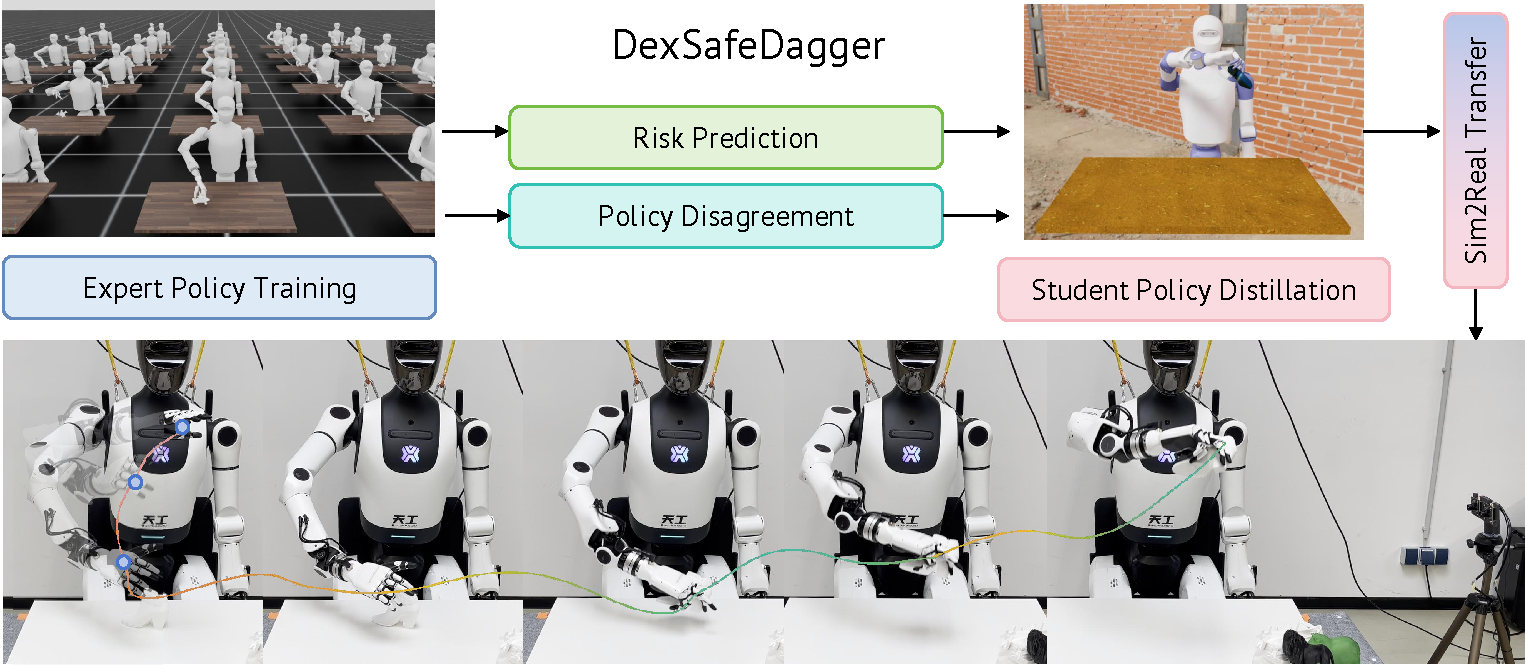
\includegraphics[width=1.0\linewidth]{figures/fig01_teaser-dexsafedagger.pdf}
%       \centering
%       % \vspace{-0.2in}
%       \captionof{figure}{Title
%       }
%       \label{fig:teaser}
%       \vspace{-0.1in}
%       \bigskip}
% \makeatother
% \maketitle

\makeatletter
\def\@onedot{\ifx\@let@token.\else.\null\fi\xspace}
\DeclareRobustCommand\onedot{\futurelet\@let@token\@onedot}
\newcommand{\figref}[1]{Fig\onedot~\ref{#1}}
\newcommand{\secref}[1]{Sec\onedot~\ref{#1}}
\newcommand{\tabref}[1]{Tab\onedot~\ref{#1}}
\def\etal{\emph{et al}\onedot}
\newcommand\ananye[1]{\textcolor{red}{#1}}

\let\@oldmaketitle\@maketitle
\renewcommand{\@maketitle}{%
  \@oldmaketitle
  \begin{center}
    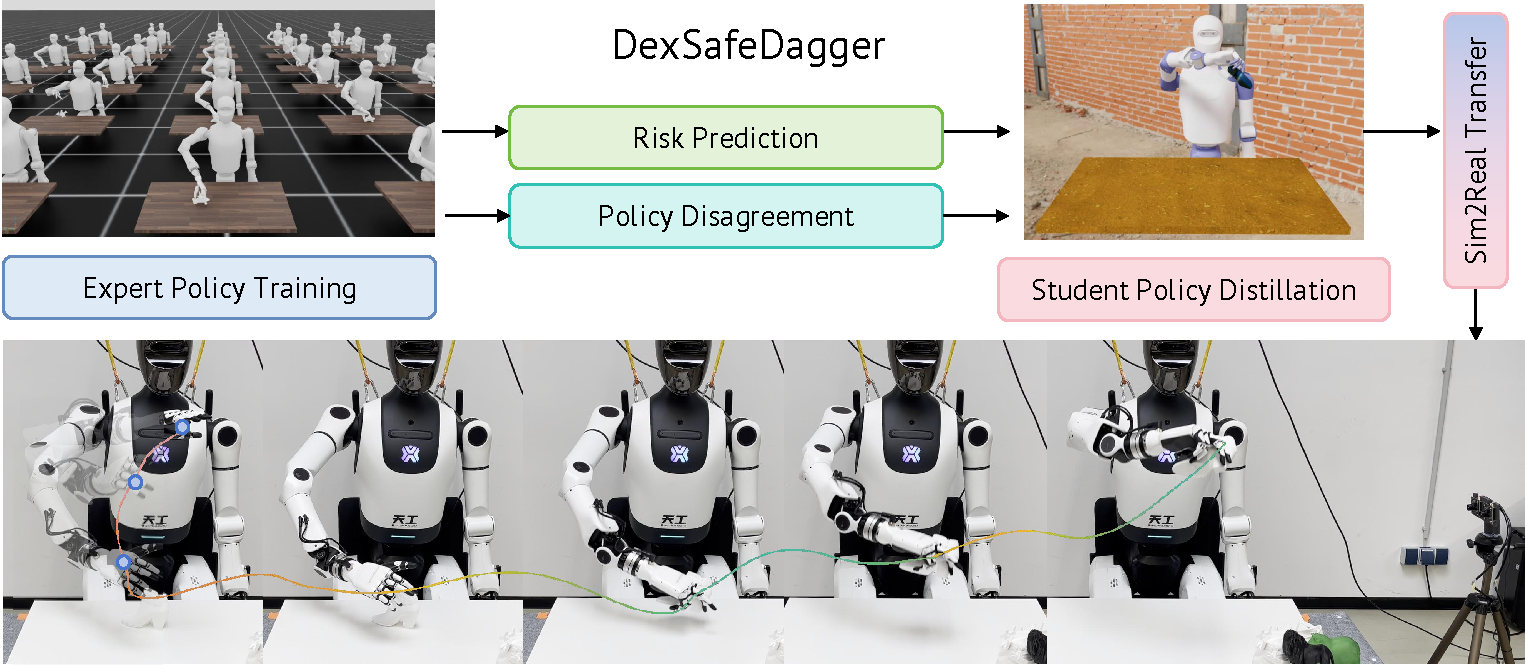
\includegraphics[width=1.0\linewidth]{figures/fig01_teaser-dexsafedagger.pdf}
    \captionof{figure}{\textbf{DexSafeDAgger overview.}
      We propose a teacher-intervened online distillation pipeline that condenses teacher skills into a
    deployable RGB-based student policy. The unsafe exploration rate is substantially suppressed in the early
    training phase via a customized
    intervention mechanism that combines teacher--student action disagreement with a learned risk predictor.}
    \label{fig:teaser}
    \vspace{-0.3in}\bigskip
  \end{center}%
}
\makeatother

% --- document body ---
\begin{document}
\maketitle

 % \thispagestyle{empty}
% \pagestyle{empty}
% \begin{document}
% \maketitle
% \thispagestyle{empty}
% \pagestyle{empty}
% \maketitle
\thispagestyle{empty}
\pagestyle{empty}
\setcounter{figure}{1}

%%%%%%%%%%%%%%%%%%%%%%%%%%%%%%%%%%%%%%%%%%%%%%%%%%%%%%%%%%%%%%%%%%%%%%%%%%%%%%%%
\begin{abstract}
% Learning dexterous manipulation is challenging due to high-dimensional action spaces and complex contact dynamics.
% Moreover, safety-unaware learning can hinder real-world deployment by increasing the risk of hardware damage,
% unstable interactions, and hazardous contact events during exploration.
% In this work, we propose a safety-aware online distillation framework that distills reinforcement learning (RL)
% teacher policies into a student policy via mixed rollouts gated by teacher--student action disagreement and a learned
% Q-value-based risk predictor. Across grasp-and-lift evaluations, the proposed method significantly reduces unsafe
% episodes (up to 80\% relative reduction early in training) while achieving a comparable lift success rate that is
% suitable for real-world deployment.

Learning dexterous manipulation is challenging due to high-dimensional action spaces and complex contact dynamics. In addition, safety-unaware exploration during learning can lead to hardware damage, unstable interactions, and hazardous contact events, posing a significant barrier to real-world deployment. 
To address this challenge, we propose a safety-aware online policy distillation framework that transfers reinforcement learning (RL) teacher policies to a vision-based student policy. Our approach introduces a teacher-intervened mixed rollout mechanism that integrates teacher–student action disagreement with a learned Q-value–based risk predictor to detect high-risk states and proactively trigger teacher takeover. This design enables safer exploration while preserving the benefits of online interactive imitation learning. 
Experiments on grasp-and-lift tasks show that our method significantly improves training safety, reducing unsafe episodes by up to 80\% during the early stages of training compared with vanilla DAgger-based distillation. Meanwhile, the distilled student policy achieves comparable lift success rates and demonstrates robustness suitable for real-world robotic deployment.
\end{abstract}


%%%%%%%%%%%%%%%%%%%%%%%%%%%%%%%%%%%%%%%%%%%%%%%%%%%%%%%%%%%%%%%%%%%%%%%%%%%%%%%%
\section{INTRODUCTION}
\label{sec:introduction}
% Dexterous robotic hands, which mimic the anthropomorphic structure of
% the human hand, typically possess a large number of degrees of freedom
% (DoFs). This high level of dexterity makes them well suited for
% complex and contact-rich tasks such as grasping (e.g., pinching,
% tripod, and power grasps) and in-hand manipulation (e.g., reorientation
% and twisting). However, this same dexterity also introduces mechanical
% delicacy and control complexity, making dexterous hands among the most
% fragile components in robotic systems, particularly in highly dynamic
% platforms such as humanoid robots. 

Dexterous robotic hands typically possess a large number of degrees of freedom (DoFs) 
and exhibit complex contact dynamics, enabling them to perform fine-grained and diverse 
manipulation behaviors, such as multi-finger grasping~\cite{brahmbhatt2019contactgrasp}, in-hand 
reorientation~\cite{chen2022system,andrychowicz2020learning}, and precise control~\cite{luo2025precise}. However, 
the high-dimensional action space and intricate interaction dynamics substantially increase 
the difficulty of control and policy learning. In recent years, reinforcement learning (RL)-based 
approaches~\cite{rajeswaran2017learning,andrychowicz2020learning,akkaya2019solving,petrenko2023dexpbt} 
have achieved remarkable progress in dexterous grasping and manipulation tasks. Leveraging large-scale 
parallel simulation and high-fidelity physics engines, RL enables the automatic learning of complex
control policies in simulated environments without the need for manually designed controllers. 
These methods have demonstrated strong generalization capabilities across multi-object and 
multi-task scenarios. 

Despite these advances, existing reinforcement learning frameworks primarily optimize for task 
success rates and rarely incorporate explicit modeling or constraints related to safety-critical 
behaviors. During training, common failure modes include severe collisions between the hand and 
the environment, unintended object ejection due to excessive contact forces, and loss of stable 
hand posture~\cite{liu2023safe,yu2022dexterous}. Such unsafe behaviors not only reduce training 
efficiency but also introduce potential risks during real-world deployment. Therefore, how to 
reduce unsafe exploration while maintaining learning efficiency remains a critical challenge in 
dexterous manipulation.

% Among the central challenges in dexterous manipulation research is how 
% to acquire reliable skills for complex systems like dexterous hands and 
% how to bridge the sim to real gap effectively. 

% Recent research has made significant progress in acquiring various skills
% through learning-based approaches. Policies can be learned
% via reinforcement learning in simulated environments conditioned with task
% specifics. Concurrent advances in vectorized simulation and increasingly realistic
% physics engines equipped with a wide range of accurate sensor choices,
% have greatly simplified the reinforcement learning process.

%====================================================
% To mitigate the performance gap between simulation and real-world deployment, policy distillation has become a widely adopted paradigm in recent years. The core idea is to first train a high-performing expert policy in simulation using privileged state information, and then distill its decision-making behavior into a student policy that relies solely on visual observations or partially observable inputs. This process enables modality transfer from privileged state information to perception-based inputs, facilitating efficient real-world deployment. 
% Policy distillation reduces reliance on accurate state estimation and allows knowledge integration from multiple teacher policies, thereby significantly improving execution stability and generalization performance in real-world environments. Consequently, it has gained increasing attention in dexterous grasping and complex manipulation tasks. 
% However, existing distillation methods~\cite{} typically rely on behavior cloning or the standard DAgger framework for data aggregation. Their primary objective is to mitigate performance degradation caused by distribution shift, rather than explicitly enforcing safety constraints during student policy learning. During distillation, the student policy may deviate from the teacher’s state–action distribution and enter regions that are either insufficiently covered by the teacher or inherently high-risk, leading to unsafe behaviors such as severe collisions or unstable hand configurations. 
% Therefore, introducing explicit safety mechanisms into the distillation process—so that high-risk exploration can be avoided without sacrificing learning efficiency—remains an important and largely underexplored problem. Existing safety-aware distillation approaches~\cite{}, such as SafeDAgger~\cite{}, have primarily focused on autonomous driving scenarios and have not been systematically studied in the context of dexterous manipulation.

To mitigate the performance gap between simulation and real-world deployment,
policy distillation has become a widely adopted paradigm in recent years. The
core idea is to first train a high-performing expert policy in simulation using
privileged state information, and then distill its decision-making behavior into
a student policy that relies solely on visual observations or partially
observable inputs. This process enables modality transfer from privileged state
information to perception-based inputs, facilitating efficient real-world
deployment.
Policy distillation reduces reliance on accurate state estimation and allows
knowledge integration from multiple teacher policies, thereby substantially
improving execution stability and generalization performance in real-world
environments. Consequently, it has gained increasing attention in dexterous
grasping and complex manipulation tasks.
However, existing distillation methods~\cite{ross2011reduction,singh2024dextrah}
typically rely on behavior cloning or the standard DAgger framework for data
aggregation. Their primary objective is to mitigate performance degradation
caused by distribution shift, rather than explicitly enforcing safety
constraints during student policy learning. During distillation, the student
policy may deviate from the teacher’s state--action distribution and enter
regions that are either insufficiently covered by the teacher or inherently
high-risk, leading to unsafe behaviors such as severe collisions or unstable
hand configurations.
Therefore, introducing explicit safety mechanisms into the distillation
process---so that high-risk exploration can be avoided without sacrificing
learning efficiency---remains an important and largely underexplored problem.
Existing safety-aware distillation
approaches, such as
SafeDAgger~\cite{zhang2016query}, have primarily focused on autonomous driving
scenarios and have not been systematically studied in the context of dexterous
manipulation.

%===================================================================================
% To address the sim-to-real transfer problem, techniques such as domain
% randomization and domain adaptation have been widely adopted. However,
% these methods often lack interpretability. In contrast, imitation learning
% has played a key role in multi-policy compression and efficient knowledge
% transfer. Among these approaches, policy distillation has attracted
% increasing research attention not only for its ability to consolidate
% multiple specialized teacher skills, but also for its potential to enable
% observation modality transfer.

% Most prior work studies policy distillation purely in simulation, where it is
% used for behavior replication or policy compression. However, both in simulation
% and in real-world deployment, student policies are limited by imperfect
% imitation and are inevitably exposed to distributional shift, visiting states
% that were not encountered during the teacher's learning process. Under such
% conditions, safe exploration of the task space is critical to avoid catastrophic
% outcomes.

% To address this challenge, we propose a pipeline that combines
% reinforcement-learning-based teacher training for per-object grasping skills
% with distillation into an RGB-based student policy. We further enhance the
% distillation process with a teacher-intervened exploration strategy, guided by a
% combined decision signal derived from both teacher--student disagreement and a
% risk-prediction probability.

The contributions of this work are summarized as follows:
\begin{itemize}
    \item We propose a safety-sensitive framework for distilling RL-acquired teacher policies into a single RGB-based
    student policy. To the best of our knowledge, this is the first attempt in dexterous manipulation to incorporate
    a mixed intervention mechanism that combines teacher--student action
    disagreement with a Bellman success-value critic trained from lift-success
    labels. Low predicted success triggers proactive teacher takeover.

    \item We propose a safety-aware RL reward design that explicitly accounts for risky events in 
    arm--hand control scenarios, including harmful collisions, object escape, palm flipping, and the hand moving 
    too far from the workspace, thereby encouraging safer exploration during teacher training.
    
    \item We empirically demonstrate that combining disagreement and success-value prediction substantially reduces unsafe
    exploration compared with vanilla DAgger, achieving a relative reduction of \textbf{80\%} in unsafe exploration
    rate in the early training phase. We also observe a \textbf{5\%} improvement in unsafe exploration rate compared
    with disagreement-only SafeDAgger.
\end{itemize}


\section{Related work}
\label{sec:related_works}
% \subsection{Reinforcement Learning for Dexterous Grasping}
% Reinforcement learning (RL) has emerged as a powerful paradigm for acquiring
% complex manipulation skills in high-degree-of-freedom (DoF) systems such as
% dexterous robotic hands. Recent research has relied heavily on model-free RL
% algorithms, including DDPG, SAC, and PPO, which have demonstrated strong
% performance in learning a variety of skills across a wide range of robotic
% setups.

% GraspXL reformulates the RL problem as an objective-conditioned
% motion generation task. The policy is trained to simultaneously
% produce stable grasps while satisfying user-specified motion
% objectives, such as graspable regions defined via signed
% distance fields (SDFs), approach directions, wrist rotations,
% and target hand poses. This formulation enables multi-objective
% policy learning within a unified reinforcement learning
% framework.

% DextrAH-RGB\cite{singh2024dextrah} adopts a geometric fabrics-based reinforcement
% learning framework, in which the policy operates within a
% hand-designed fabric-induced action manifold. This structured
% representation effectively reduces the action-space dimension
% and significantly simplifies reward design during training.

\textbf{Skill Distillation.} Skill distillation transfers behavior from a high-capacity teacher to a compact student and has been widely adopted
in both computer vision and robotics. In robotics, the teacher can leverage privileged state and simulator access during training,
while the student is distilled to operate from on-board observations (e.g., RGB). DexTrAH-RGB~\cite{singh2024dextrah} 
distills a privileged RL teacher into an RGB-based policy via DAgger-based imitation learning, while 
UniGraspTransformer~\cite{wang2025unigrasptransformer} distills offline trajectories from object-specific teachers 
into a unified Transformer policy.

\textbf{Adaptive Intervention in Interactive Imitation Learning.} Many imitation learning methods use fixed offline datasets for supervision~\cite{zhang2025contactdexnet,zhang2025omnidexvlg}. In sequential decision-making, however, distribution shift induces covariate shift and compounding errors. Interactive imitation learning~\cite{welte2025interactive} mitigates these issues by collecting online supervision along trajectories visited by the learner.
DAgger~\cite{ross2011reduction} addresses covariate shift by iteratively relabeling learner-visited states with an expert, while SafeDAgger~\cite{zhang2016query} adds teacher intervention in high-risk states to reduce unsafe exploration.

Later methods introduce adaptive intervention mechanisms based on uncertainty-driven rules~\cite{menda2019ensembledagger}, human gating~\cite{kelly2019hgdagger}, or learned intervention criteria~\cite{cai2025robot}. However, they have primarily been evaluated in relatively simple control or autonomous-driving settings. Fully autonomous expert relabeling during online distillation remains rare in robotic manipulation,
especially for dexterous, contact-rich tasks.

\textbf{Vision-Language-Guided Robot Learning.}
Visual and semantic information is widely recognized as a strong 
cue for embodied agents to interpret task specifications and reason 
about unstructured environments~\cite{firoozi2025foundation,han2026multimodal}.
One line of work uses VLMs to generate demonstrations or supervisory signals
for offline policy construction, such as
Manipulate-Anything~\cite{duan2025manipulate}.
Complementary approaches, including RACER~\cite{dai2025racer} and
FOREWARN~\cite{wu2025foresight}, employ VLMs to guide risk prediction,
provide recovery guidance for unsafe situations, or govern action selection
during online policy learning or real-time execution.

\section{Problem Statement and Methods}\label{sec:method}

\begin{figure*}[t]
    \centering
    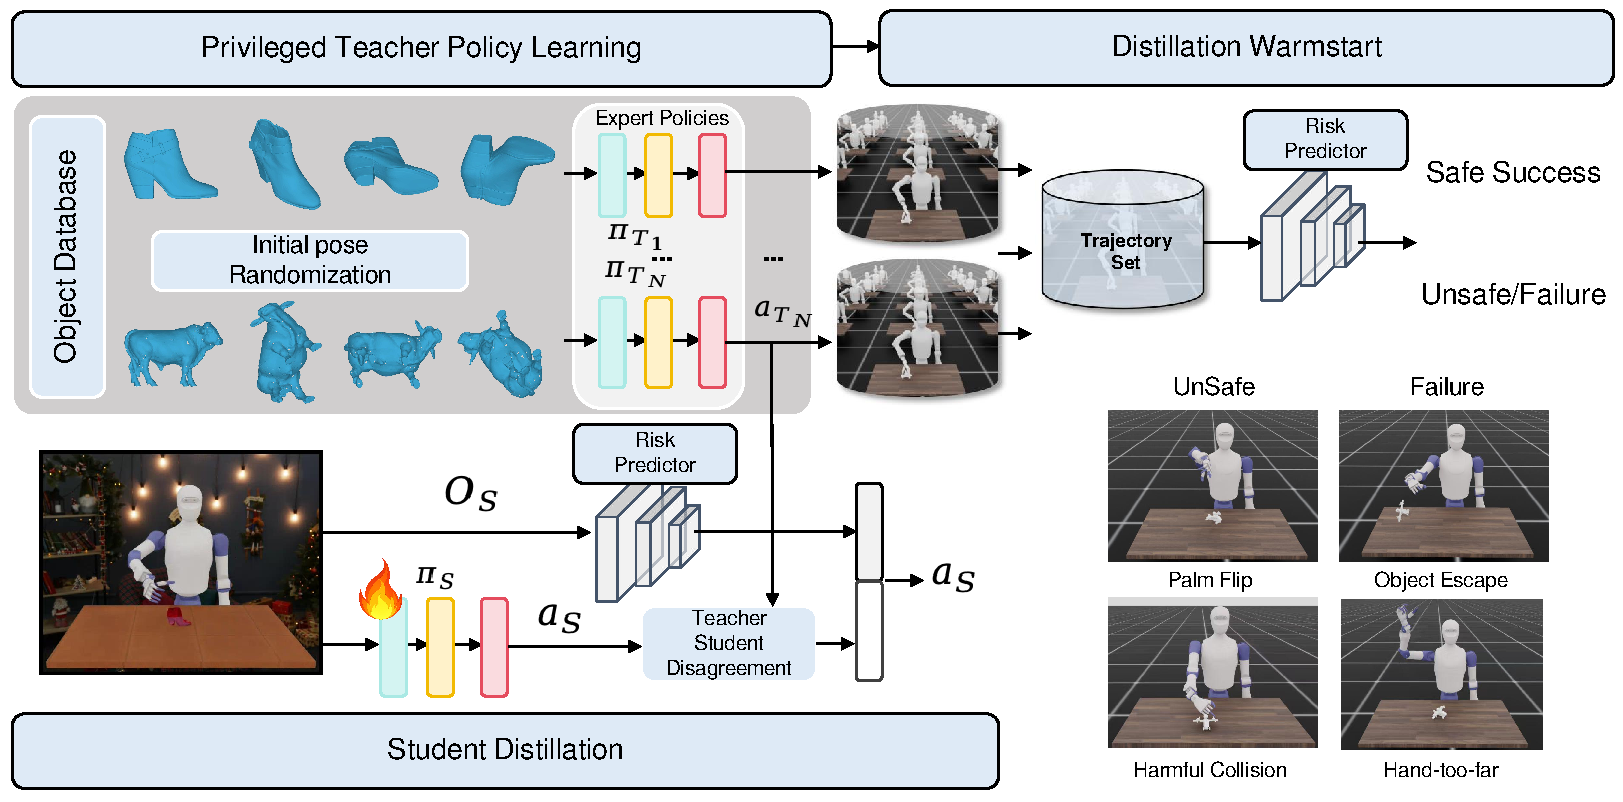
\includegraphics[width=0.8\linewidth]{figures/fig02_network_structure.pdf}
    \par\redtodo{TODO: Update Figure 2.}
    \caption{Overview of the proposed teacher--student learning pipeline. A
    privileged reinforcement learning teacher is trained in simulation and
    subsequently distilled into an RGB-based visuomotor policy for real-world
    deployment. \revision{A vision-language model periodically calibrates the
    intervention thresholds.}}
    \label{fig:pipeline}
\end{figure*}

\subsection{Problem Formulation}
We consider online interactive imitation learning with teacher intervention in a
partially observable Markov decision process (POMDP)
$\mathcal{M}=(\mathcal{S},\mathcal{A},\mathcal{O},P,\Omega,r,\gamma)$, with
privileged teacher state $s_t\in\mathcal{S}$, deployable student observation
$o_t\in\mathcal{O}$ (RGB), action $a_t\in\mathcal{A}$, observation model
$o_t\sim\Omega(\cdot\mid s_t)$, and dynamics
$s_{t+1}\sim P(\cdot\mid s_t,a_t)$. During training, we assume access to a set
of privileged teacher policies $\{\pi_{T_i}\}_{i=1}^{K}$, whereas at deployment
the student policy $\pi_S$ must act solely from $o_t$. Our goal is to distill
the collective teacher behavior into an RGB-based student that achieves high
task success while minimizing unsafe exploration during training.

The induced rollout distribution $p_{\pi_{\mathcal{G}}}$ is defined by the gated rollout policy
$\pi_{\mathcal{G}}$, which switches between the teacher and student policies
according to the intervention gate. Its learning objective and VLM-calibrated
gate are
\begingroup
\small
\begin{equation}
\begin{aligned}
\min_{\substack{\pi_S\in\Pi_S\\ \mathcal{G}\in\mathfrak{G}}}
\;
&
\Bigg[
\underbrace{
-\mathbb{E}_{\tau\sim p_{\pi_{\mathcal{G}}}}\!\left[\mathbb{I}_{\mathrm{succ}}(\tau)\right]
}_{\text{maximize success}}
\;+\;
\lambda\,
\underbrace{
\mathbb{E}_{\tau\sim p_{\pi_{\mathcal{G}}}}\!\left[
\sum_{t=0}^{T-1}\mathbb{I}_{\mathrm{unsafe}}(s_t,a_t)
\right]}_{\text{minimize unsafe}}
\Bigg]
\\
\text{s.t.}\quad
&
a_t=g_t a_t^T+(1-g_t)a_t^S,\\
&
g_t=\mathcal{G}(s_t,o_t)\in\{0,1\},\\
&
s_{t+1}\sim P(\cdot\mid s_t,a_t),\qquad
o_t\sim\Omega(\cdot\mid s_t).
\end{aligned}
\label{eq:vc_objective}
\end{equation}
\endgroup
where $g_t=1$ indicates teacher takeover and $g_t=0$ denotes student control.
\revision{The intervention gate $\mathcal{G}$ and its VLM-calibrated thresholds
are described in Secs.~E--F.}

We formalize task success via a trajectory-level predicate
$\mathbb{I}_{\mathrm{succ}}(\tau)\in\{0,1\}$, which is $1$ if the object is
grasped, lifted, and held above a height threshold for a consecutive duration.
Safety is governed by early termination conditions: letting
$\mathbb{I}_{\mathrm{unsafe}}(s_t,a_t)\in\{0,1\}$ indicate whether any unsafe
event (e.g., harmful collision, object escape, palm flip, hand-too-far) occurs
at time $t$, the trajectory is safe if
$\prod_{t=0}^{T-1}\big(1-\mathbb{I}_{\mathrm{unsafe}}(s_t)\big)=1$.

\subsection{Overview of the Distillation Pipeline}
Fig.~\ref{fig:pipeline} summarizes our teacher--student distillation pipeline,
which consists of three core components: (i) privileged teacher policy training
in simulation (Sec.~C), (ii) risk predictor learning to estimate lift success
under student actions (Sec.~D), and (iii) online student distillation with
teacher intervention (Secs.~E and G). \revision{We additionally introduce a VLM
tuner (Sec.~F) that periodically calibrates the intervention thresholds.} We
warm-start the risk predictor using an offline dataset collected under full
teacher control and continue updating it periodically during online
distillation using mini-batches sampled from a ring replay buffer. During
interactive rollouts, an intervention gate $\mathcal{G}$ switches control
between teacher and student based on an OR-rule combining a learned risk
estimate and teacher--student action disagreement. The student is then
optimized online using per-timestep teacher labels collected under the gated
rollout policy $\pi_{\mathcal{G}}$. \revision{At a slower timescale, the VLM
reviews rollout statistics and representative visual states and proposes
conservative threshold updates.} Pseudo-code is provided in
Alg.~\ref{alg:safe_dagger}.

\begin{algorithm}[t]
\small
\caption{Safe Policy Distillation with Risk-Guided Teacher Intervention}
\label{alg:safe_dagger}
\begin{algorithmic}[1]

\STATE Train teacher policy $\pi_T$ via reinforcement learning
\STATE Collect offline dataset $\mathcal{D}_0$ using $\pi_T$
\STATE Pretrain risk predictor $\hat{Q}(s,a)$ on $\mathcal{D}_0$

\FOR{iteration $k = 1 \dots N$}

    \STATE Observe student observation $o_t$
    \STATE Compute student action $a^S_t \sim \pi_S(\cdot|o_t)$
    \STATE Query teacher action $a^T_t \sim \pi_T(\cdot|s_t)$
    
    \STATE Compute disagreement $\delta_t = \|a^S_t - a^T_t\|_2$
    \STATE Evaluate risk score $\hat{Q}(s_t, a^S_t)$

    \IF{$d_t > \tau_D$ \textbf{or} $\hat{Q}(s_t,a^S_t) < \tau_{\text{success}}$}
        \STATE Execute teacher action $a_t = a^T_t$
    \ELSE
        \STATE Execute student action $a_t = a^S_t$
    \ENDIF

    \STATE Store $(o_t, a^T_t)$ in ring replay buffer $\mathcal{D}$
    \STATE Update student policy $\pi_S$ via imitation loss
    \STATE Update risk predictor $\hat{Q}$ using replay buffer

\ENDFOR

\end{algorithmic}
\end{algorithm}

\subsection{Privileged Teacher Policy Training}
Teacher policy learning is formulated as a reinforcement learning problem with
transition tuples $\langle s_t,a_t,r_t,s_{t+1}\rangle$, where $s_t$ is the
privileged state, $a_t$ is the action, $r_t$ is the reward, and $s_{t+1}$ is the
next state. The objective is to maximize the expected discounted return,
\begingroup
\small
\begin{equation}
\pi_T^*
=
\arg\max_{\pi_T}\;
\mathbb{E}_{\pi_T}
\left[
\sum_{t=0}^{T-1}\gamma^t r_t
\right].
\label{eq:teacher_rl_objective}
\end{equation}
\endgroup
We use a shaped reward $r_t=\sum_{k=1}^{K_r} r_{t,k}$ to encourage stable grasp
acquisition, object lifting, and goal reaching (Table~\ref{tab:reward_terms}).

The teacher is trained in simulation using an asymmetric actor--critic setup
(Table~\ref{tab:teacher_obs}): the actor receives noisy and partial
proprioceptive observations that approximate realistic sensing, while the
critic is provided with privileged full state of both robot and object,
available only in simulation.

\begin{table}[t]
\centering
\footnotesize
\caption{Reward components used for teacher policy training.}
\label{tab:reward_terms}
\setlength{\tabcolsep}{3pt}
\renewcommand{\arraystretch}{0.9}
\resizebox{0.46\textwidth}{!}{%

\begin{tabularx}{\columnwidth}{@{}c l X@{}}
\hline
\textbf{Term} & \textbf{Name} & \textbf{Purpose} \\
\hline
$r_{\text{dist}}$ & Hand distance &
Guides the hand toward the object. \\

$r_{\text{curl}}$ & Finger curl &
Encourages a grasp-ready finger posture. \\

$r_{\text{align}}$ & Palm alignment &
Aligns the palm to a palm-down pose. \\

$r_{\text{contact}}$ & Contact bonus &
Rewards stable thumb--finger contact. \\

$r_{\text{near}}$ & Stay-close &
Keeps the hand near the object after reaching. \\

$r_{\text{goal}}$ & Goal tracking &
Guides the grasped object toward the goal. \\

$r_{\text{lift}}$ & Lift &
Rewards lifting after stable contact. \\

$r_{\text{action}}$ & Action smoothness &
Penalizes abrupt action changes. \\
\hline
\end{tabularx}
}
\end{table}


Episodes terminate at
\begingroup
\small
\begin{equation}
T = \min\left\{t \,\middle|\, \mathbb{I}_{\mathrm{unsafe}}(s_t)=1
\;\;\text{or}\;\; t \ge T_{\max}\right\},
\end{equation}
\endgroup
where $T_{\max}=10\,\mathrm{s}$ is the timeout horizon. Early termination
conditions include palm flip, harmful collision, object escape, and hand-too-far
(see Sec.~A), and are treated as unsafe events for both teacher training and
subsequent intervention decisions.

\subsection{Risk Predictor}
Action disagreement alone cannot anticipate downstream failures, particularly
when the student action is locally similar to the teacher action yet triggers
unstable contact transitions. To address this limitation, we learn a risk
predictor that conservatively estimates the probability of \emph{lift success}.
The predictor is used only during training to guide teacher intervention and is
not required at deployment time.

The risk predictor is designed to estimate risk from multimodal inputs. It
takes as input a state--action pair $(s_t,a_t)$, where $s_t$ comprises robot
proprioceptive features concatenated with image embeddings produced by a visual
encoder to provide semantic information. The visual encoder is trained
end-to-end during distillation and regularized via an auxiliary object-position
prediction loss (Sec.~G). The action $a_t$ is the \emph{executed} action at time
$t$ (teacher or student, depending on the intervention gate). Following a
clipped double-critic design, we maintain two critics $Q_1$ and $Q_2$
implemented as ReLU MLPs with hidden sizes $[256,128]$, each outputting a scalar
logit $z_i(s,a)\in\mathbb{R}$ mapped to a success probability via a
temperature-calibrated sigmoid,
$Q_i(s,a)=\sigma\!\left(z_i(s,a)/T\right)$ for $i\in\{1,2\}$, where $T=4$ is an
empirically set calibration temperature. We then compute
\begingroup
\small
\begin{equation}
\hat Q_{\mathrm{succ}}(s,a)=\min\!\left(Q_1(s,a),\,Q_2(s,a)\right),
\label{eq:success_critic}
\end{equation}
\endgroup
which provides a conservative estimate of lift success (lower values indicate
higher risk).

The predictor is pretrained in a warm-start phase using an offline dataset of
transitions $(s_t,a_t,s_{t+1},a_{t+1},u_t,d_t,h_t)$. Here, $(s_t,a_t)$ and
$(s_{t+1},a_{t+1})$ provide the current and next state--action pairs required by
SARSA-style bootstrapping, $d_t\in\{0,1\}$ is the episode termination flag, and
$h_t\in\{0,1\}$ indicates whether the next action $a_{t+1}$ is defined (valid)
for bootstrapping. The label $u_t\in\{0,1\}$ encodes \emph{safe lift-event}
attainment by time $t$: $u_t=1$ if the object has been lifted above a height
threshold for a consecutive duration (as in $\mathbb{I}_{\mathrm{succ}}$) and no
unsafe event has occurred up to time $t$; otherwise $u_t=0$.

During online distillation, newly collected transitions are appended to a ring
buffer (sized $100k$) at every environment step. The predictor critics are
updated periodically: every $500$ environment steps, we perform $20$ gradient
updates using mini-batches sampled from the buffer using Adam with learning
rate $10^{-3}$.

Training uses SARSA-style bootstrapped regression with an effective termination
signal $d_t^{\mathrm{eff}}=\max(d_t,1-h_t)$ and one-step target
\begingroup
\small
\begin{equation}
y_t=
\operatorname{clip}\!\left(
u_t+\gamma(1-d_t^{\mathrm{eff}})
\min_{i\in\{1,2\}}Q_i^{\mathrm{targ}}(s_{t+1},a_{t+1}),
\,0,\,1\right),
\label{eq:success_target}
\end{equation}
\endgroup
where $Q_i^{\mathrm{targ}}$ are slowly-updated target networks (Polyak
averaging) used only to stabilize bootstrapping, and the $\min$ operator
mitigates overestimation. The critics are optimized with MSE
$\mathcal{L}_{Q_i}=\mathbb{E}\!\left[
w_t\big(Q_i(s_t,a_t)-y_t\big)^2\right]$, with total loss
$\mathcal{L}=\mathcal{L}_{Q_1}+\mathcal{L}_{Q_2}$ and target updates
$\theta'\leftarrow\rho\theta'+(1-\rho)\theta$ ($\rho=0.995$).

During interactive distillation, the predictor estimates the task success
probability of executing the \emph{student} action: given $s_t$ and
$a_t^S\sim\pi_S(\cdot\mid o_t)$, we compute
$\hat Q_{\mathrm{succ}}(s_t,a_t^S)$ and trigger teacher takeover when it falls
below a threshold (Sec.~E).

\subsection{Intervention Mechanism}
At each timestep, we compute (i) a risk score using the learned predictor and
(ii) a teacher--student disagreement score. Disagreement is defined as
$\delta_t\coloneqq\lVert a_t^S-a_t^T\rVert_2$, where
$a_t^T\sim\pi_T(\cdot\mid s_t)$ and $a_t^S\sim\pi_S(\cdot\mid o_t)$ are the
teacher and student action outputs. The risk criterion flags states whose
predicted success under the student action is low, i.e.,
$\hat Q_{\mathrm{succ}}(s_t,a_t^S)<\tau_Q^{(k)}$.

We instantiate the intervention gate $\mathcal{G}$ as an OR-rule that triggers
teacher takeover when either the predictor indicates high risk or the student
deviates substantially from the teacher:
\begingroup
\color{yellow!50!black}
\begingroup
\small
\begin{equation}
g_t=
\mathbb{I}\!\left[
\hat Q_{\mathrm{succ}}(s_t,a_t^S)<\tau_Q^{(k)}
\;\lor\;\delta_t>\tau_{\delta}^{(k)}
\right],
\label{eq:adaptive_gate}
\end{equation}
\endgroup
where $k$ indexes the latest calibration update. Intuitively, disagreement
detects distribution shift, while the risk predictor anticipates downstream
failures even when the instantaneous action discrepancy is small.
\endgroup

\revision{We initialize $\tau_\delta^{(0)}$ to the $90$th percentile of the
teacher--student disagreement $\delta_t$ measured on the warm-start dataset.
We initialize $\tau_Q^{(0)}$ to a low percentile (e.g., the $10$th) of
$\hat Q_{\mathrm{succ}}(s_t,a_t^T)$ computed over successful warm-start
rollouts. These percentiles provide base thresholds chosen empirically to
balance intervention frequency and exploration efficiency; the VLM tuner
subsequently calibrates them during training (Sec.~F).}

\begingroup
\color{yellow!50!black}
\subsection{VLM Threshold Tuner}
\label{subsec:vlm_threshold_tuner}

To adapt the arbitration rule to non-stationary learning dynamics, we introduce
a vision-language-model (VLM) based threshold tuner. The tuner periodically
calibrates the two thresholds in Eq.~\eqref{eq:adaptive_gate} as both the
student policy and the visited-state distribution evolve during data
aggregation. At iteration $k$, the VLM is provided with rollout-level summary
statistics
$\mathcal{C}_k$, including the teacher--student disagreement, predicted
success, intervention frequency, and unsafe-event rate. In addition, it receives
a small set of representative visual observations corresponding to
high-disagreement, low-success, and unsafe states. These visual examples provide
context about the failure modes encountered by the student, while the scalar
statistics summarize the global behavior of the current policy.

The VLM is used as a high-level calibration module. It recommends candidate
thresholds
$(\tilde{\tau}_{\delta}^{(k)},\tilde{\tau}_{Q}^{(k)})$. To avoid abrupt changes, each proposed threshold is constrained around its initial value
and then exponentially smoothed:
\begin{equation}
\begin{aligned}
\tau_{x}^{(k+1)}
&=(1-\alpha)\tau_{x}^{(k)}
+\alpha\,\operatorname{clip}\!\left(
\tilde{\tau}_{x}^{(k)},
c_{x}^{\min}\tau_{x}^{0},
c_{x}^{\max}\tau_{x}^{0}\right),\\[-2pt]
&\hspace{5.5em}x\in\{\delta,Q\}.
\end{aligned}
\label{eq:vlm_threshold_update}
\end{equation}
Here, $\alpha$ controls the adaptation rate, while
$c_{x}^{\min}$ and $c_{x}^{\max}$ define the admissible range relative to the
initial threshold $\tau_x^0$.  
\endgroup


\subsection{Student Policy Distillation}
Student learning is posed as supervised imitation from teacher-labeled
transitions collected under the gated rollout policy $\pi_{\mathcal{G}}$. The
student observes RGB images (two stereo views) together with robot proprioception.

We optimize a combined objective
$\mathcal{L}=\mathcal{L}_{\mathrm{action}}+\mathcal{L}_{\mathrm{aux}}$, where the
auxiliary loss predicts object position to regularize the visual encoder,
$\mathcal{L}_{\mathrm{aux}}=\lVert
\hat{\mathbf{x}}_{\mathrm{obj}}-\mathbf{x}_{\mathrm{obj}}\rVert_2$.

For action imitation, we use a weighted $L_2$ loss,
$\mathcal{L}_{\mathrm{action}}
=\lVert\mathbf{a}_S-\mathbf{a}_T\rVert_W^2
=(\mathbf{a}_S-\mathbf{a}_T)^\top W(\mathbf{a}_S-\mathbf{a}_T)$,
with $W=\mathrm{diag}(w_1,\dots,w_d)$. We set
$w_j=\sigma_{0,j}^{-2}$ using a reference scale $\sigma_{0,j}$ (e.g., the
teacher action standard deviation on dimension $j$), yielding
$\mathcal{L}_{\mathrm{action}}=
\sum_{j=1}^{d}(a_{S,j}-a_{T,j})^2/\sigma_{0,j}^{2}$.

Training proceeds in two stages. (i) \emph{Warm-start:} we collect an offline
dataset (e.g., $100$k transitions) under full teacher control ($g_t\equiv 1$)
to pretrain the risk predictor. (ii) \emph{Online
distillation:} we perform interactive rollouts under $\pi_{\mathcal{G}}$ and
query teacher labels on intervened steps. The student is updated online using
the current-step teacher label only; we do \emph{not} maintain a replay buffer
or DAgger-style aggregated dataset for student updating. The design reduces the
effect of stale supervision and stabilizes online imitation updates.


\section{Experiment}
\label{sec:experiment}
\subsection{Evaluation Metrics}
We designed the following metrics to evaluate both teacher and student policy performance.
Let $\tau\in\{1,\dots,N\}$ index evaluation episodes and $t\in\{0,\dots,T_\tau\}$ index timesteps.
Unless otherwise stated, we run the evaluation episodes with a horizon of 10\,s.

\paragraph{Lift success (ever-lifted with hold).}
Let $h_t^\tau$ be the object height above the table and $H$ a lift threshold. An episode is considered
successful if the object remains above $H$ for at least $N_{\mathrm{hold}}$ consecutive steps. We define
$\mathbb{I}^{\tau}_{\mathrm{lift}}
=\mathbb{I}\!\left[\exists\, t:\ \forall k\in\{0,\dots,N_{\mathrm{hold}}-1\},\ h_{t+k}^{\tau}\ge H\right]$
and report:
$\mathrm{LiftSucc}=\frac{1}{N}\sum_{\tau=1}^{N} \mathbb{I}^{\tau}_{\mathrm{lift}}.$

\paragraph{Unsafe episode rate.}
As stated above, an episode may terminate early due to one of the following conditions:
palm flipped ($\mathbb{I}_{\mathrm{flip}}^{\tau}$), harmful collision ($\mathbb{I}_{\mathrm{coll}}^{\tau}$),
object escape ($\mathbb{I}_{\mathrm{obj}}^{\tau}$), or hand too far ($\mathbb{I}_{\mathrm{hf}}^{\tau}$).
Let $\mathcal{M}=\{\mathrm{coll},\mathrm{obj},\mathrm{flip},\mathrm{hf}\}$ denote the set of termination modes,
and let $\mathbb{I}_m^\tau\in\{0,1\}$ indicate whether mode $m\in\mathcal{M}$ occurs in episode $\tau$.
An episode is unsafe if any termination mode is triggered:
$\mathbb{I}^{\tau}_{\mathrm{unsafe}}
=\mathbb{I}\!\left[\bigvee_{m\in\mathcal{M}} \mathbb{I}^{\tau}_{m}=1\right]$. We report:
$\mathrm{UnsafeRateAvg}=\frac{1}{N}\sum_{\tau=1}^{N} \mathbb{I}^{\tau}_{\mathrm{unsafe}}.$

\paragraph{Failure-mode decomposition.}
Each episode is assigned a single terminal mode $m^\tau\in\mathcal{M}$ from the
set of unsafe events (collision, object escape, palm flip, hand-too-far) as well
as timeout/success where applicable. We define
$\mathbb{I}^{\tau}_{m}=\mathbb{I}[m^\tau=m]$ and report
$\mathrm{FailureModeRate}(m)=\frac{1}{N}\sum_{\tau=1}^{N}\mathbb{I}^{\tau}_{m}, m\in\mathcal{M}.$

When multiple unsafe conditions are triggered in the same timestep, we record
the first triggered termination condition (using a fixed priority order) as the
episode's failure mode.

\subsection{Simulation Experiment Setup}

\begin{figure*}[t]
    \centering
    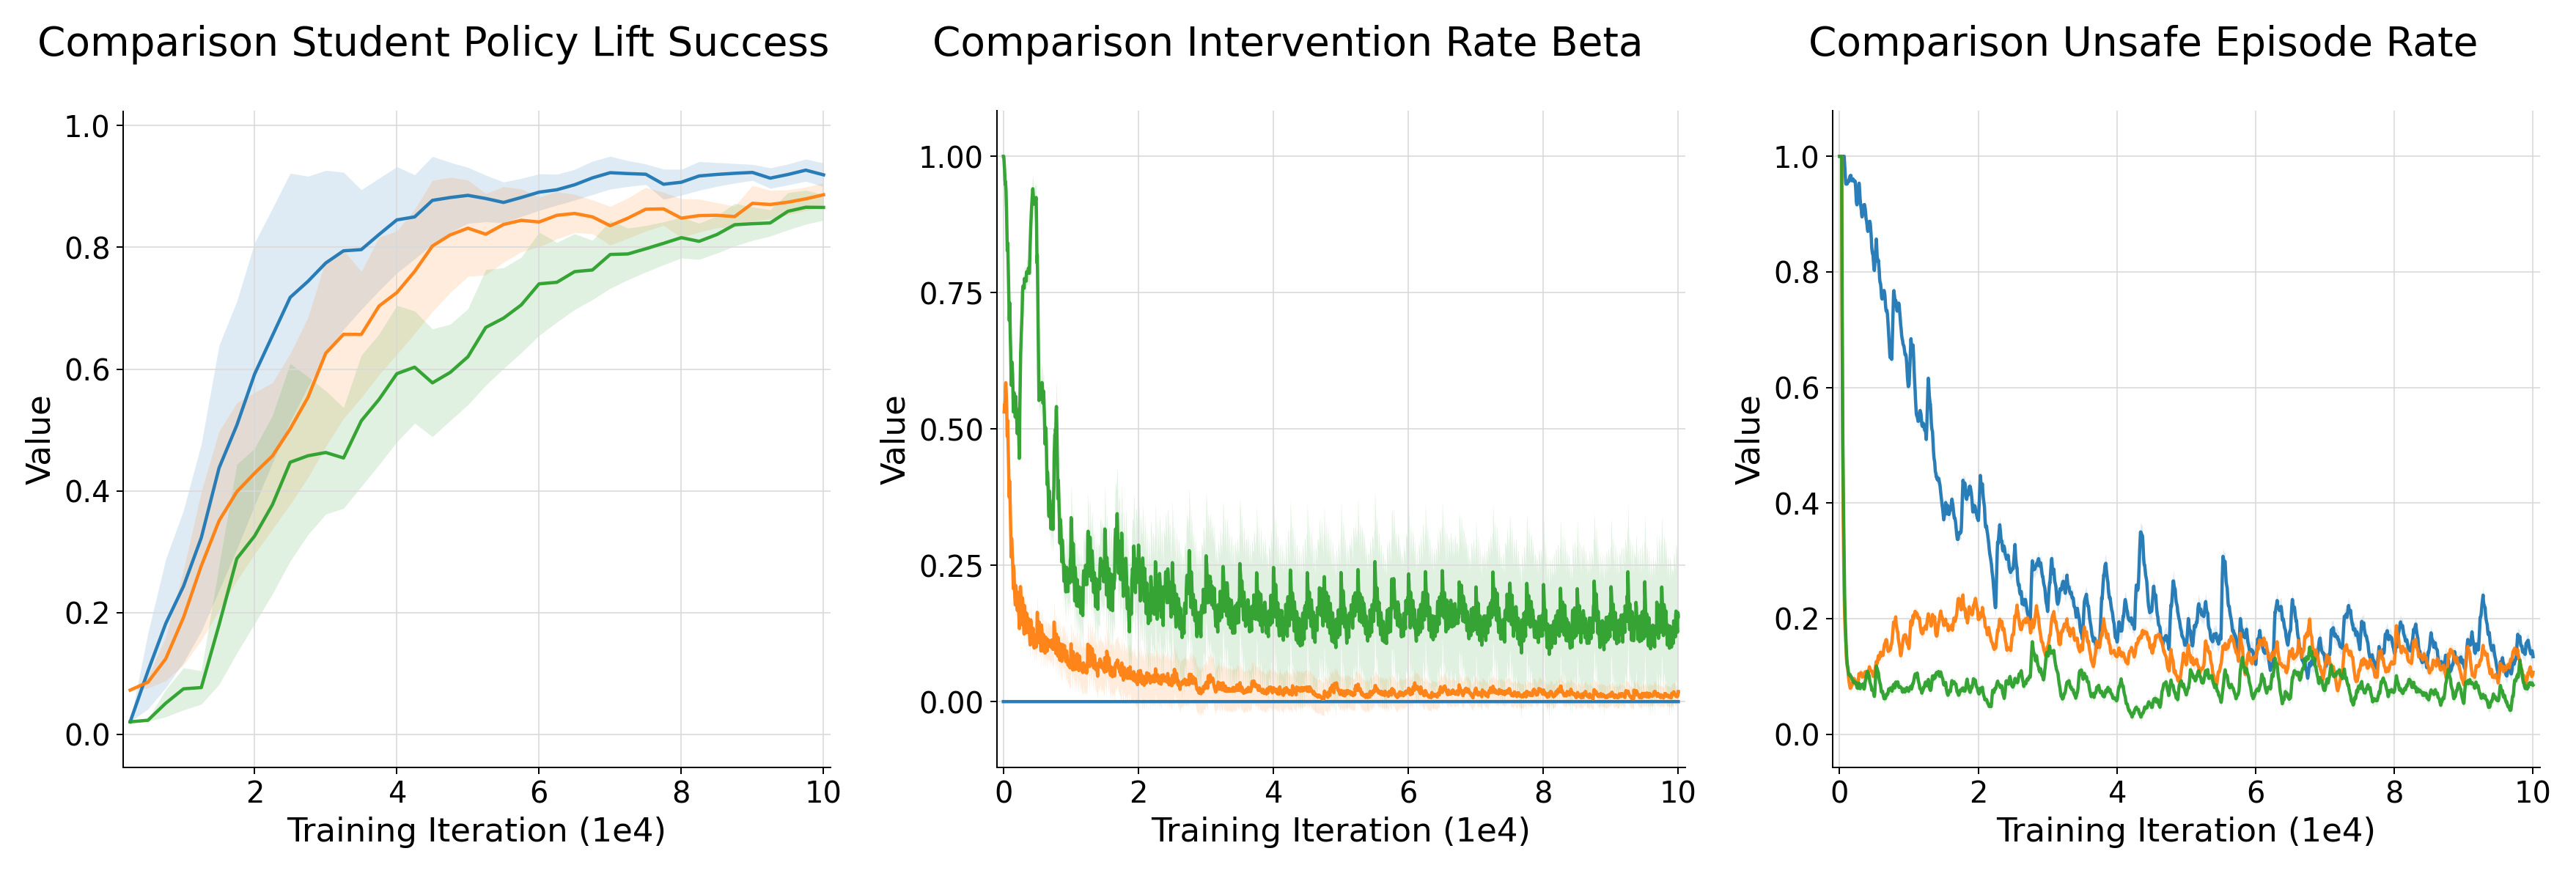
\includegraphics[width=\linewidth]{figures/ablation_comparison.png}
    \caption{\textbf{Ablation studies.}
    The first three panels compare four distillation variants in terms of student lift success, teacher intervention rate $\beta$, and unsafe episode rate, respectively, all plotted over training iterations.
    The rightmost panel shows the VLM-guided trajectory of the intervention operating point over online training.
    Shaded regions indicate variability across runs (mean $\pm$ std).
    Curves correspond to vanilla DAgger (blue), vanilla SafeDAgger (orange),
    \dexsafedagger (green), and \methodname (red).}
    \label{fig:ablation}
\end{figure*}

% The simulation experiments are based on single-arm control of a Tiangong~2 Pro
% humanoid robot equipped with InspireHand RH56DfX dexterous hands. The action
% space is 13-dimensional, consisting of 7 DoF for the robotic arm and 6 DoF for
% the dexterous hand.

% The student policy additionally receives image streams from two cameras at a
% resolution of $320\times240$ pixels and $30$\,fps. The raw stereo images are
% encoded by a visual encoder into a 64-D embedding, which is appended to the
% teacher actor observations to form the student observation. Concretely, the
% visual encoder uses a shared (Siamese) ResNet-18 backbone (last two layers
% removed) for each view, followed by an MLP projection and a 2-layer
% cross-attention transformer to fuse the two views; the resulting
% token is mapped to the 128-dimensional visual feature vector.

% Both teacher policy training and student skill distillation are conducted in Isaac Sim 5.0.0 and
% Isaac Lab 2.2.1 on a single NVIDIA RTX~5090 GPU.

% Forty objects sourced from the Omniverse Asset Library are tested in total. Each teacher policy is trained for 12{,}000 episodes,
% requiring approximately 3.5~hours. The teacher policies achieve a lift success rate ranging from 68\% to 
% 100\% and an unsafe rate ranging from 5\% to 30\%. The results are reported in Table~3.

% During student skill distillation, lighting intensity, direction and background textures are randomized at the
% beginning of each episode. Furthermore, object material properties, textures, and table appearance are randomized to encourage
% improved sim-to-real transfer, following a setup similar to DexTrAH-RGB. The distillation phase requires approximately 2.5~hours to complete
% 100{,}000 episodes.

Simulation experiments use single-arm control on a Tiangong~2 Pro humanoid equipped with InspireHand RH56DfX; the action
space is 13-D (7 arm DoF + 6 hand DoF). The RGB student additionally receives two $320\times240$ camera streams at
30\,fps, encoded by a Siamese ResNet-18 visual backbone with view fusion into a 128-D feature appended to the actor
observation. Teacher training and student distillation are conducted in Isaac Sim 5.0.0 / Isaac Lab 2.2.1 on a single
RTX~5090 GPU.

We evaluate 40 objects from the Omniverse Asset Library and train one
object-specific teacher for each object. Each teacher is trained for
12{,}000 episodes (3.5\,h), totaling 480{,}000 teacher-training
episodes and approximately 140 GPU-hours. Across the 40 teachers, lift-success
rates range from 72--100\%, and unsafe rates range from 5--30\%;
Table~\ref{tab:teacher_perf_200} reports a representative four-object subset.
During distillation, we randomize lighting intensity, direction, background
textures, object material, and table appearance following DexTrAH-RGB-style
domain randomization. The joint student is distilled across all 40 objects for
100{,}000 episodes in 2.5\,h. 

We use GPT-5.5 with high reasoning effort as the VLM. We issue the first VLM
query after 2{,}000 episodes
and subsequently query it every 10{,}000 distillation episodes, resulting in 10
VLM calls over the full 100{,}000-episode training run and approximately
70{,}000 tokens of total usage per run.

% \begin{table}[t]
\centering
\small
\caption{Observation spaces used for teacher RL training under the
asymmetric actor--critic framework.}
\label{tab:teacher_obs}
\resizebox{0.38\textwidth}{!}{%
\begin{tabular}{lcc}
\hline
\textbf{Observation Component} & \textbf{Actor} & \textbf{Critic} \\
\hline
Robot DOF positions  & 13 (noisy) & 13 \\
Robot DOF velocities  & 13 (noisy) & 13 \\
Hand link positions & 18 & 18 \\
Hand link velocities & 18 & 36 (twist) \\
Hand contact forces & -- & 3 \\
Measured joint torque & -- & 19 \\
Object position & 3 & 3 \\
Object rotation (quaternion) & 4 & 4 \\
Object velocity & -- & 6 (twist) \\
Goal position & 3 & 3 \\
Object scale & 1 & 1 \\
Previous actions & 13 & 13 \\
\hline
\textbf{Total dimension} & \textbf{86} & \textbf{132} \\
\hline
\end{tabular}
}
\end{table}

\begin{table}[t]
\centering
\small
\caption{Teacher policy performance on four representative objects from the
40-object training set (200 evaluation episodes per object).}
\label{tab:teacher_perf_200}
\setlength{\tabcolsep}{4pt}
\renewcommand{\arraystretch}{1.2}
\resizebox{0.38\textwidth}{!}{%

\begin{tabular}{l|cccc|c}
\hline
Metric (\%) & WindCart & Boot & ToolBox & Cow & \textbf{Mean} \\
\hline
Lift Success         & 93.5 & 100.0 & 88.5 & 87.0 & 92.3 \\
Unsafe Rate Avg      & 6.5   & 13.5  & 13.5 & 13.5 & 11.8 \\
Harmful collision    & 0.0   & 0.0   & 6.5  & 0.0  & 1.6  \\
Object escape        & 6.5   & 6.5   & 6.5  & 13.5 & 8.3  \\
Palm flipped         & 0.0   & 6.5   & 0.0  & 0.0  & 1.6  \\
Hand too far         & 0.0   & 0.0   & 0.0  & 0.0  & 0.0  \\
\hline
\end{tabular}
}
\end{table}


\subsection{Ablation Studies}

We perform the following ablation studies to validate the design choices in
\methodname and answer four questions: \textbf{(i)~Does our customized RL
recipe produce stronger teachers than the DexTrAH-RGB-style training recipe?}
\textbf{(ii)~Does the intervention mechanism in \dexsafedagger enable safer
exploration during policy distillation?} \textbf{(iii)~Does augmenting action
disagreement with success-value prediction improve the intervention signal?}
\textbf{(iv)~Is visual-language reasoning necessary for adapting the
intervention boundary?}

% \noindent\textbf{(a) DexTrAH-RGB RL teacher + Vanilla DAgger.}
% We follow the DexTrAH-RGB teacher training setup and distill the resulting teacher into a student using
% Vanilla DAgger. Rollouts in simulation are fully controlled by the student policy, while the teacher runs
% in parallel in the background with the intervention rate $\beta$ fixed to $0$. At each timestep, the
% executed student action $a_t^{S}$ is relabeled with the corresponding teacher action $a_t^{T}$.

\noindent\textbf{(a) DexTrAH-RGB RL + Vanilla DAgger.}
The teacher is trained using the DexTrAH-RGB RL recipe and then distilled into
a student policy using supervision only, with no teacher intervention during
rollouts ($\beta=0$).

% \noindent\textbf{(b) Our RL teacher + Vanilla DAgger.}
% We replace the DexTrAH-RGB teacher training pipeline with our customized RL recipe and use the same
% Vanilla DAgger-style online distillation.

\noindent\textbf{(b) Our RL + Vanilla DAgger.}
This setting matches (a), except that our RL recipe replaces the DexTrAH-RGB
teacher-training recipe.

% \noindent\textbf{(c) Our RL teacher + Vanilla SafeDAgger.}
% The teacher policy is trained using our RL pipeline, and we extend Vanilla DAgger to a Vanilla SafeDAgger
% distillation setup. The student and teacher policies are rolled out in parallel, and the teacher action takes
% over only when the $\ell_2$ distance between the teacher and student actions exceeds a threshold, indicating
% a large teacher--student disagreement. The student is trained on teacher-labeled pairs $(o_t^{S}, a_t^{T})$,
% where $o_t^{S}$ denotes the student observation.

\noindent\textbf{(c) Our RL + Vanilla SafeDAgger.}
The teacher training follows the recipe in (b), but we replace Vanilla DAgger
with a disagreement-gated SafeDAgger baseline. The teacher intervenes only when
$\lVert a_t^{T}-a_t^{S}\rVert_2$ exceeds a fixed threshold.

% \noindent\textbf{(d) DexTrAH-RGB RL teacher + SafeDAgger with disagreement and a success-value critic.}
% We follow the DexTrAH-RGB teacher training setup but apply our teacher-intervened distillation pipeline for
% student learning. The teacher and student policies are rolled out in parallel. Teacher intervention is triggered
% when either (i) the teacher disagrees with the student or (ii) the success-value critic flags the current transition
% as unlikely to lead to task success. The intervention decision is computed at every timestep. Likewise, the
% student is trained on teacher-labeled pairs $(o_t^{S}, a_t^{T})$.

\noindent\textbf{(d) DexTrAH-RGB RL + \dexsafedagger.}
We use the teacher-training recipe from (a) and the intervention baseline from
(c), extending it with a Bellman success-value critic under a stationary
intervention policy. Teacher intervention is triggered by either large
teacher--student disagreement or low predicted success.

% \noindent\textbf{(e) Our RL teacher + SafeDAgger with disagreement and a success-value critic.}
% We combine our custom RL pipeline with the proposed teacher intervention mechanism, using both teacher--student
% disagreement and success-value prediction to trigger teacher takeover.

\noindent\textbf{(e) Our RL + \dexsafedagger.}
Following the recipe in (d), we replace the teacher-training pipeline with our
customized RL recipe.

\noindent\textbf{(f) Our RL + \methodname.}
This setting extends (e) by replacing the stationary intervention policy with
the proposed VLM tuner, which periodically calibrates the disagreement-risk
intervention policy using rollout statistics and representative visual states.

\noindent\textbf{(g) Our RL + LLM-DexSafeDagger.}
This setting matches (f), except that the language model receives only the
rollout statistics and no visual observations.

\noindent\textbf{(h) Our RL + Grid-Search \dexsafedagger.}
This setting replaces the language/vision model in (f) with grid search over
the intervention thresholds. The remaining teacher, student, success-value
critic, and distillation components are held fixed.

To answer question~(i), we compare (a) with (b) and (d) with (e). The
DexTrAH-RGB-style RL recipe achieves lower performance than our RL recipe. We
attribute this gap to the specialized tuning of the \textsc{Fabrics} controller
for the original task setup, which transfers poorly to new hardware and
dynamics.

\begin{table}[t]
\centering
\small
\caption{Performance of ablations (a)--(h) on four representative objects from the
40-object training set (200 evaluation episodes per object). Each ablation
reports lift success and average unsafe rate.}
\label{tab:ablation_studies}
\setlength{\tabcolsep}{3pt}
\renewcommand{\arraystretch}{1.15}
\resizebox{0.48\textwidth}{!}{%
\begin{tabular}{l|cc|cc|cc|cc|cc}
\hline
\multirow{2}{*}{Metric (\%)}
& \multicolumn{2}{c|}{WindCart}
& \multicolumn{2}{c|}{Boot}
& \multicolumn{2}{c|}{ToolBox}
& \multicolumn{2}{c|}{Cow}
& \multicolumn{2}{c}{\revisionadded{\textbf{Mean}}} \\
\cline{2-11}
& Lift  & Unsafe
& Lift  & Unsafe
& Lift  & Unsafe
& Lift  & Unsafe
& \revisionadded{Lift}  & \revisionadded{Unsafe}  \\
\hline
\textbf{(a)} & 75.0 & 24.0 & 76.5 & 28.0 & 72.0 & 26.0 & 70.0 & 27.5 & \revisionadded{72.7} & \revisionadded{26.5} \\
\textbf{(b)} & 88.5 & 13.5 & 89.0 & 20.5 & 82.5 & 19.0 & 88.0 & 17.5 & \revisionadded{87.1} & \revisionadded{17.4} \\
\textbf{(c)} & 88.0 & 12.0 & 89.5 & 19.5 & 81.5 & 18.5 & 87.0 & 16.0 & \revisionadded{86.3} & \revisionadded{16.7} \\
\textbf{(d)} & 74.5 & 23.0 & 75.0 & 27.5 & 70.5 & 26.5 & 69.5 & 27.0 & \revisionadded{72.3} & \revisionadded{25.8} \\
\textbf{(e)} & 88.0 & 7.5 & 90.0 & 15.0 & 82.0 & 15.5 & 88.0 & 12.0 & \revisionadded{86.8} & \revisionadded{11.9} \\
\textbf{(f)} & 88.5 & 6.0 & 90.0 & 10.5 & 82.5 & 11.0 & 88.5 & 8.5 & \revisionadded{87.5} & \revisionadded{9.3} \\
\revisionadded{\textbf{(g)}} & \revisionadded{88.0} & \revisionadded{7.5} & \revisionadded{89.5} & \revisionadded{12.5} & \revisionadded{82.0} & \revisionadded{13.0} & \revisionadded{88.0} & \revisionadded{10.5} & \revisionadded{86.9} & \revisionadded{10.2} \\
\revisionadded{\textbf{(h)}} & \revisionadded{86.5} & \revisionadded{7.0} & \revisionadded{88.5} & \revisionadded{14.0} & \revisionadded{81.0} & \revisionadded{13.5} & \revisionadded{87.0} & \revisionadded{11.0} & \revisionadded{85.7} & \revisionadded{11.7} \\
\hline
\end{tabular}
}
\end{table}


\begin{figure*}[!t]
    \centering
    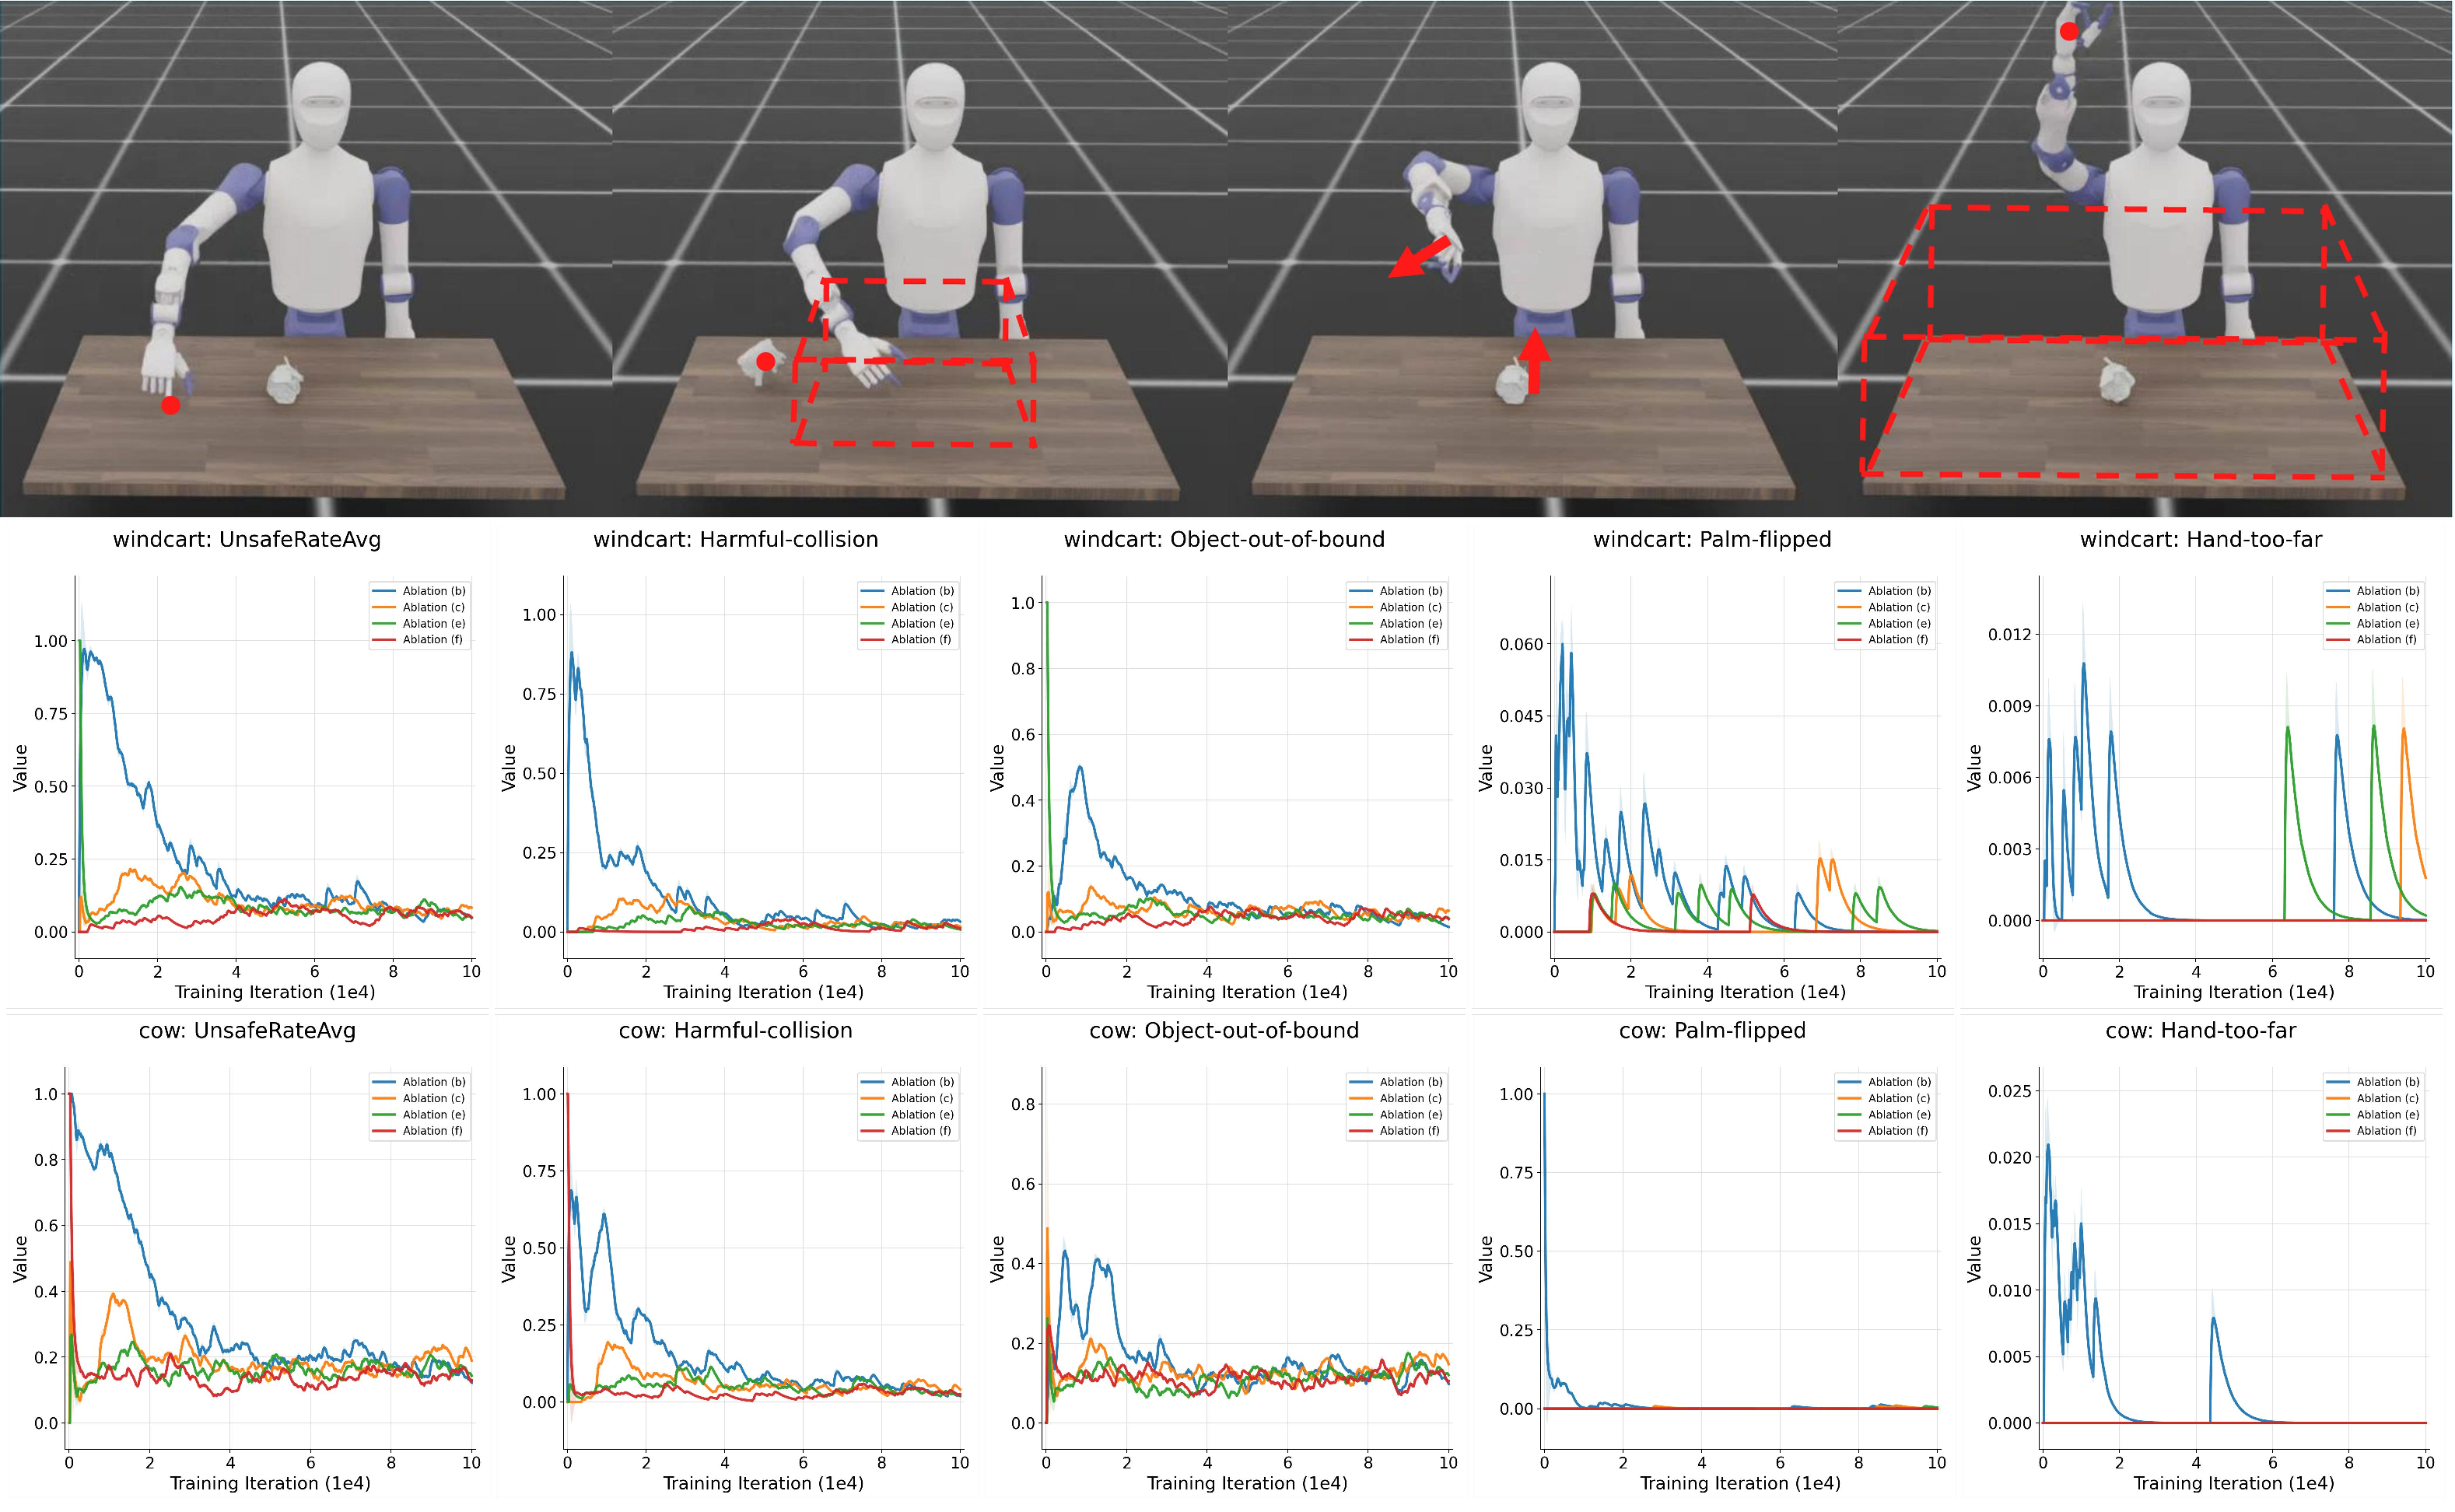
\includegraphics[width=0.82\linewidth]{figures/failure_mode.pdf}
    \caption{\textbf{Per-object failure-mode decomposition during online distillation ablations.}
    We illustrate four task-specific failure modes in simulation (harmful collision, object escape, palm flipped, and hand too far) and report the aggregate unsafe rate together with its per-mode breakdown over training iterations.
    Results are shown for two objects (\texttt{windcart} and \texttt{cow}); lower is better in all plots.
    Curves correspond to four distillation variants: blue, Vanilla DAgger\cite{ross2011reduction};
    orange, Vanilla SafeDAgger\cite{zhang2016query}; green, \dexsafedagger;
    and red, \methodname.}
    \label{fig:failure_modes}
\end{figure*}

We next address question~(ii) by examining the distillation behavior in
Fig.~\ref{fig:ablation}. Ablations (b), (c),
(e), and (f) achieve comparable final lift success
(left), consistent with the intervention policy's focus on safety rather than task success. Unlike
Vanilla DAgger ($\beta=0$), the three intervention variants reduce teacher intervention as the student
improves (middle). They reduce early unsafe episodes by approximately 80\% relative to Vanilla DAgger and
remain below 20\% throughout distillation, with \methodname achieving the lowest rate overall (right).

We address question~(iii) by comparing ablation (c), which uses disagreement alone,
with ablation (e), which adds success-value prediction
while retaining the same RL teacher and stationary intervention policy. The combined gate
intervenes in low-predicted-success states missed by disagreement alone, reducing the average
unsafe-episode rate by about 7.5 percentage points and limiting collision and object-escape
failures without sacrificing task performance. Its unsafe rate approaches the teacher's
average ($\approx 12\%$) by the end of training and reaches a minimum of approximately 8\%.
Fig.~\ref{fig:failure_modes} further shows that harmful collisions and object
escape dominate unsafe episodes. Compared with Vanilla DAgger, all three
intervention variants suppress both failure modes, particularly their early
spikes, demonstrating that teacher intervention limits unsafe exploration
during the initial distillation phase.

\begin{figure}[!t]
    \centering
    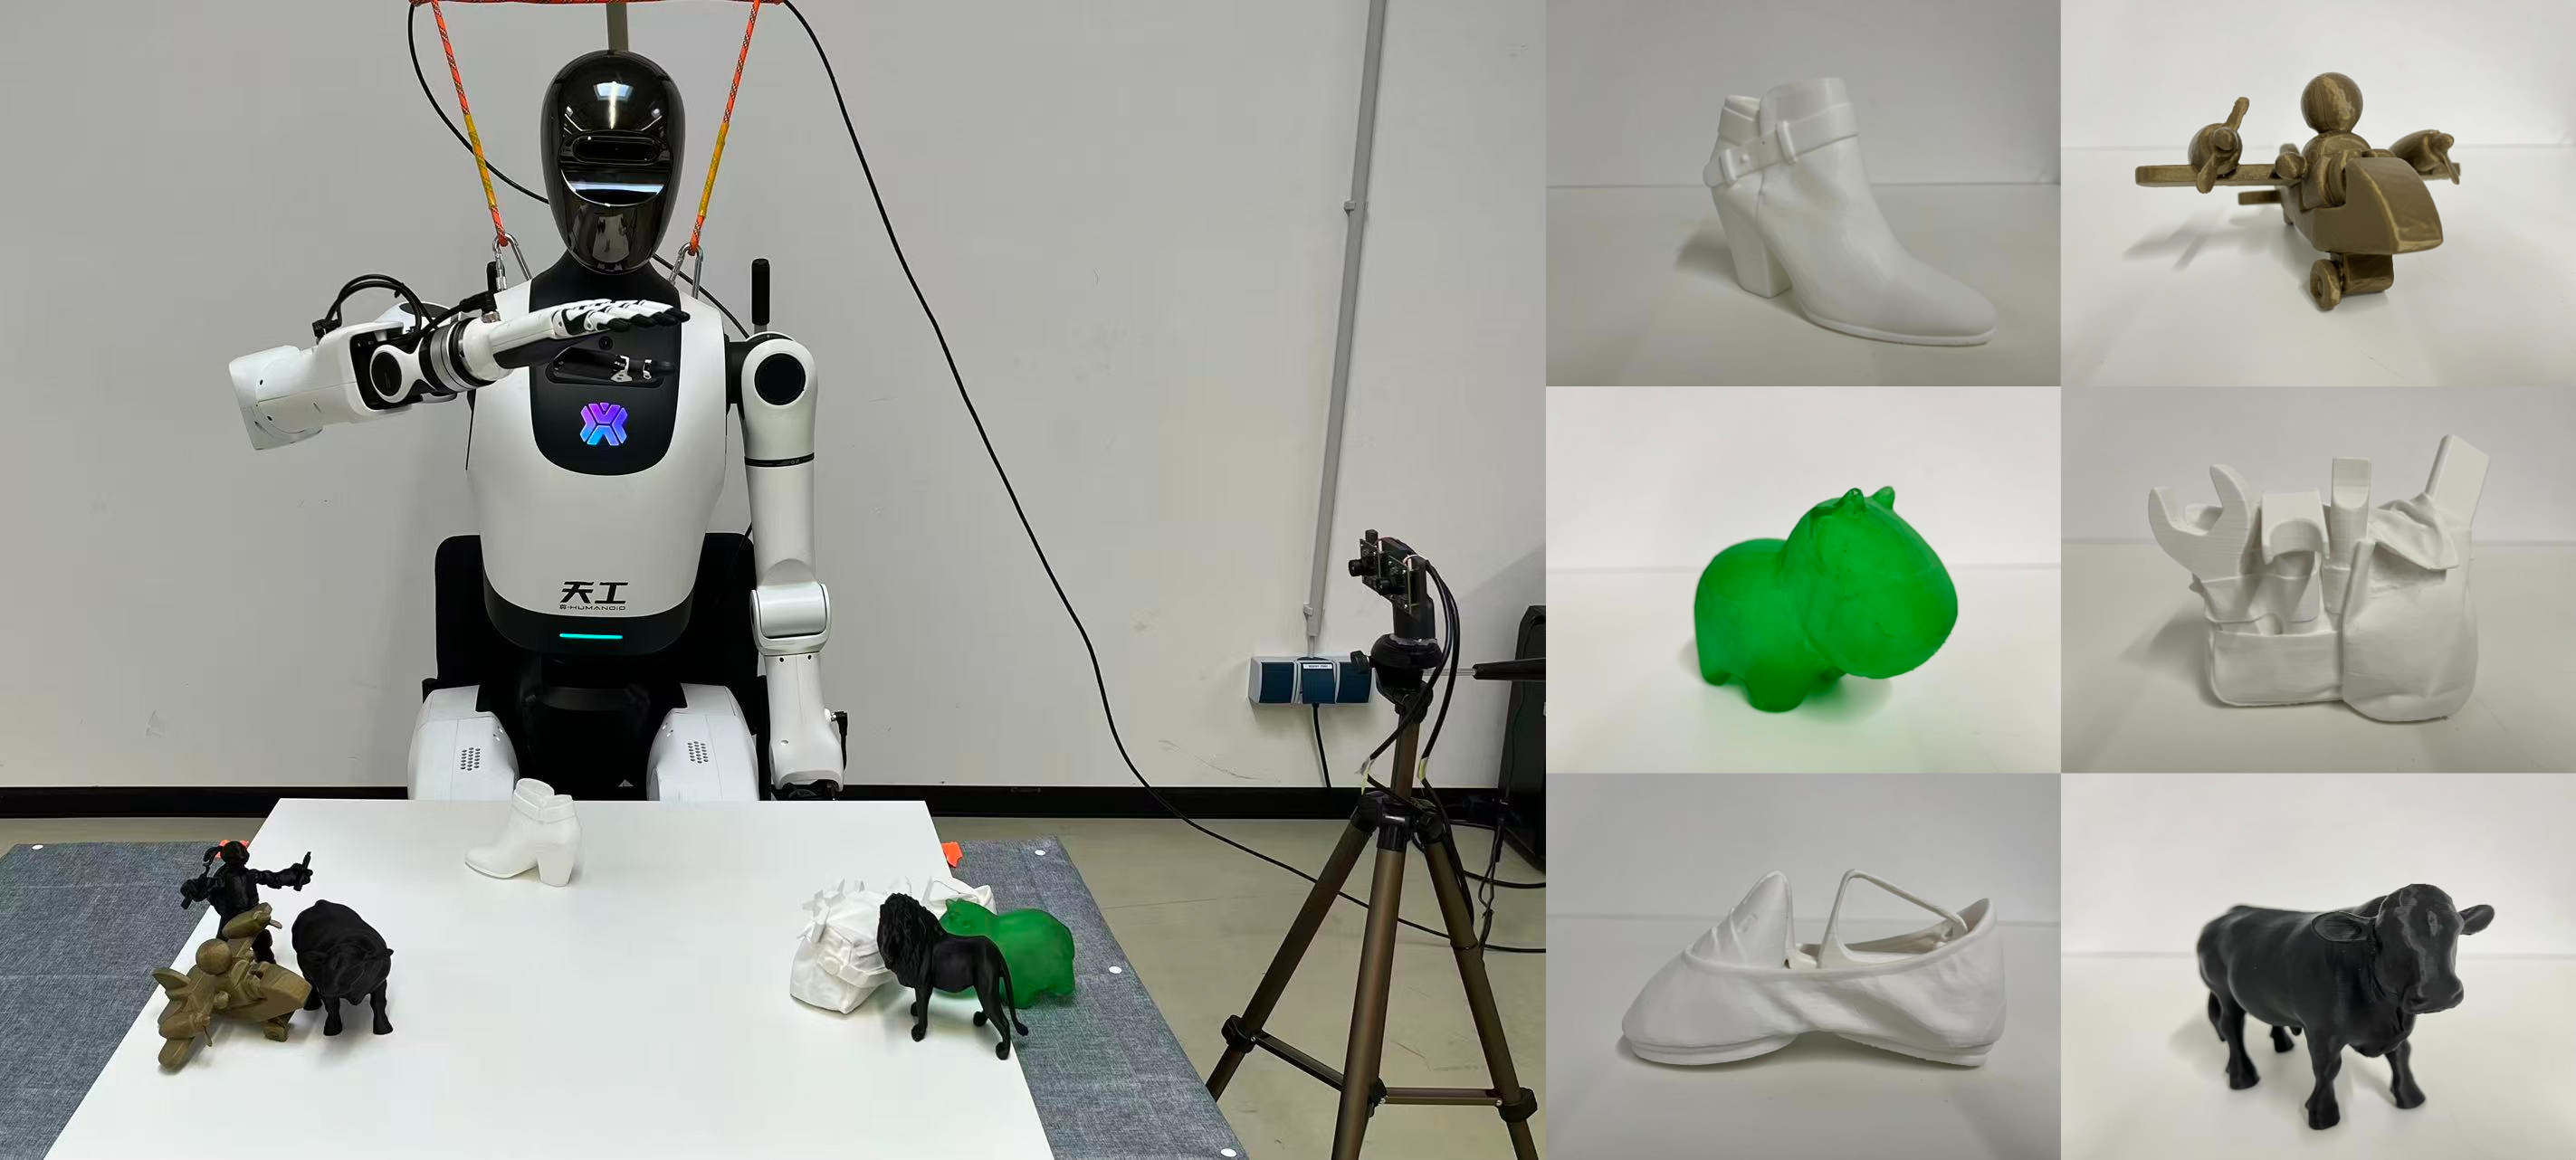
\includegraphics[width=0.85\linewidth]{figures/real_setup_1.png}
    \caption{\textbf{Real-world experimental setup and test objects.}
    Left: the single-arm manipulation platform used for deployment and evaluation.
    Right: examples of the physical objects used in the real-world lift experiments.}
    \label{fig:realworld_exp_setup}
\end{figure}

Finally, we address question~(iv) by comparing ablations (e), (h), (g), and
(f), which form a progression from stationary intervention, to grid-searched
thresholds, to semantics-guided LLM adaptation, and finally to our VLM-guided
recipe. This controlled ladder isolates the contributions of threshold
adaptation, semantic reasoning, and visual context.
\textcolor{red}{TODO: Add the quantitative comparison of ablations (e), (h),
(g), and (f) when the evaluation results are available.}
Across all evaluated
objects, ablation (f) achieves an unsafe-episode rate that is lower than that
of (e) by an average of 4 percentage points, while maintaining comparable lift
success. This result shows that VLM-guided intervention-policy adaptation
improves safety without sacrificing task performance.

\subsection{Real-World Experimental Results}

We evaluate the deployed student policy on 22 objects, comprising 16 seen objects and 6 unseen objects.
Table~\ref{tab:real_world_results} reports a representative six-object subset
and pooled results for the four seen and two unseen objects shown.
The experiments exhibit a lower lift success rate and a higher unsafe episode rate than
the teacher and student evaluation results in simulation, indicating that \methodname does
not fully eliminate the sim-to-real gap. Nevertheless, the resulting policy is sufficiently robust
for real-world deployment.

The unseen-object evaluation reveals a clear generalization gap: compared with
the seen objects shown, the policy's pooled lift success decreases from
\textcolor{red}{85.0\%} to \textcolor{red}{63.3\%}, while its unsafe rate
increases from \textcolor{red}{20.0\%} to \textcolor{red}{40.0\%} on the unseen
objects shown. This degradation is
primarily driven by increased harmful collisions (20.0\% and 26.7\% on Plane and
Shoe), while object escape remains comparable across objects
($\approx$6.7--20.0\%). No palm-flip or hand-too-far events are observed,
suggesting that real-world failures are dominated by contact-rich interactions
rather than gross pose instabilities. Overall, the results indicate that the
remaining sim-to-real gap on unseen geometries is largely attributable to a
contact-strategy mismatch, i.e., the policy fails to adapt its contact
interactions to novel object shapes.

\newcommand{\unseen}[1]{\cellcolor{gray!15}\textbf{#1}}

\begin{table}[t]
\centering
\small
\caption{Representative six-object subset of the 22-object real-world evaluation
(30 episodes per object). The last two columns report pooled results over the
complete sets of 16 seen and 6 unseen objects, respectively. \unseen{Unseen
objects} are shaded.}
\label{tab:real_world_results}
\setlength{\tabcolsep}{4pt}
\renewcommand{\arraystretch}{1.2}
\resizebox{0.48\textwidth}{!}{%

\begin{tabular}{l|cccccc|cc}
\hline
Metric (\%) & WindCart & Boot & ToolBox & Cow & \unseen{Plane} & \unseen{Shoe}
& \makecell{{\textbf{Seen}} \\ {\textbf{avg. (16)}}}
& \unseen{{\makecell{Unseen \\ avg. (6)}}} \\
\hline
Lift Success         & 87.0 & 86.3 & 80.0 & 86.7 & \unseen{66.7} & \unseen{60.0} & 86.2 & \unseen{63.9} \\
Unsafe Rate Avg      & 13.3 & 19.7 & 20.0 & 25.7 & \unseen{40.0} & \unseen{40.0} & 21.2 & \unseen{34.8} \\
Harmful collision    & 0.0  & 6.7  & 13.0 & 13.3 & \unseen{20.0} & \unseen{26.7} & 9.3  & \unseen{20.1} \\
Object escape        & 13.3 & 13.0 & 7.0  & 12.7 & \unseen{20.0} & \unseen{13.3} & 11.9 & \unseen{13.8} \\
Palm flipped         & 0.0  & 0.0  & 0.0  & 0.0  & \unseen{0.0}  & \unseen{0.0}  & 0.0 & \unseen{0.2}  \\
Hand too far         & 0.0  & 0.0  & 0.0  & 0.0  & \unseen{0.0}  & \unseen{0.0}  & 0.0  & \unseen{0.7}  \\
\hline
\end{tabular}
}
\end{table}


% \subsection{Discussion}

% While effectively reducing unsafe exploration, the teacher-intervened online distillation process
% appears to reduce sample efficiency. In Fig.~\ref{fig:ablation}, we observe slower performance growth in
% lift-success evaluation under higher intervention rates. The underlying cause remains unclear; we believe
% there is room for improvement in both exploration safety and sample efficiency within the online
% distillation paradigm.
\label{sec4:expriments}

\section{Conclusion and Future Work}
\label{sec:conclusion}
In this work, we propose \methodname, which integrates
teacher--student disagreement with a Bellman success-value critic trained on
safe-lift-success labels and uses a VLM to adapt the intervention policy.
\methodname improves exploration safety during multi-teacher distillation,
reducing the unsafe-episode rate by \textbf{80\%} relative to the vanilla DAgger
baseline during early training. The introduction of the Bellman critic
reduces the average unsafe-episode rate by \textbf{7.5 percentage points} relative to the
disagreement-only SafeDAgger baseline. In addition, VLM-guided intervention policy adaptation
yields consistent improvements across different visual contexts and unsafe scenarios,
reducing the average unsafe-episode rate by a further \textbf{4 percentage points} relative to
\dexsafedagger.
The proposed method approaches and, in some cases, surpasses the teacher policy's
safety performance. Successful real-world deployment shows that the resulting
student policy partially bridges the sim-to-real gap.

A clear limitation is that performance during distillation, as well as the final student policy, is
largely constrained by teacher capability. Developing a safety-aware teacher training pipeline is a
promising direction for future work to generate stronger teacher policies.


\vspace{0.1in}
% \noindent\textbf{Acknowledgement}

%%%%%%%%%%%%%%%%%%%%%%%%%%%%%%%%%%%%%%%%%%%%%%%%%%%%%%%%%%%%%%%%%%%%%%%%%%%%%%%%



%%%%%%%%%%%%%%%%%%%%%%%%%%%%%%%%%%%%%%%%%%%%%%%%%%%%%%%%%%%%%%%%%%%%%%%%%%%%%%%%



%%%%%%%%%%%%%%%%%%%%%%%%%%%%%%%%%%%%%%%%%%%%%%%%%%%%%%%%%%%%%%%%%%%%%%%%%%%%%%%%
% \section*{APPENDIX}

% Appendixes should appear before the acknowledgment.

% \section*{ACKNOWLEDGMENT}

% The preferred spelling of the word ÒacknowledgmentÓ in America is without an ÒeÓ after the ÒgÓ. Avoid the stilted expression, ÒOne of us (R. B. G.) thanks . . .Ó  Instead, try ÒR. B. G. thanksÓ. Put sponsor acknowledgments in the unnumbered footnote on the first page.



%%%%%%%%%%%%%%%%%%%%%%%%%%%%%%%%%%%%%%%%%%%%%%%%%%%%%%%%%%%%%%%%%%%%%%%%%%%%%%%%

% References are important to the reader; therefore, each citation must be complete and correct. If at all possible, references should be commonly available publications.


% \section{Introduction}
% % Dexterous robotic hands, which mimic the anthropomorphic structure of
% the human hand, typically possess a large number of degrees of freedom
% (DoFs). This high level of dexterity makes them well suited for
% complex and contact-rich tasks such as grasping (e.g., pinching,
% tripod, and power grasps) and in-hand manipulation (e.g., reorientation
% and twisting). However, this same dexterity also introduces mechanical
% delicacy and control complexity, making dexterous hands among the most
% fragile components in robotic systems, particularly in highly dynamic
% platforms such as humanoid robots. 

Dexterous robotic hands typically possess a large number of degrees of freedom (DoFs) 
and exhibit complex contact dynamics, enabling them to perform fine-grained and diverse 
manipulation behaviors, such as multi-finger grasping~\cite{brahmbhatt2019contactgrasp}, in-hand 
reorientation~\cite{chen2022system,andrychowicz2020learning}, and precise control~\cite{luo2025precise}. However, 
the high-dimensional action space and intricate interaction dynamics substantially increase 
the difficulty of control and policy learning. In recent years, reinforcement learning (RL)-based 
approaches~\cite{rajeswaran2017learning,andrychowicz2020learning,akkaya2019solving,petrenko2023dexpbt} 
have achieved remarkable progress in dexterous grasping and manipulation tasks. Leveraging large-scale 
parallel simulation and high-fidelity physics engines, RL enables the automatic learning of complex
control policies in simulated environments without the need for manually designed controllers. 
These methods have demonstrated strong generalization capabilities across multi-object and 
multi-task scenarios. 

Despite these advances, existing reinforcement learning frameworks primarily optimize for task 
success rates and rarely incorporate explicit modeling or constraints related to safety-critical 
behaviors. During training, common failure modes include severe collisions between the hand and 
the environment, unintended object ejection due to excessive contact forces, and loss of stable 
hand posture~\cite{liu2023safe,yu2022dexterous}. Such unsafe behaviors not only reduce training 
efficiency but also introduce potential risks during real-world deployment. Therefore, how to 
reduce unsafe exploration while maintaining learning efficiency remains a critical challenge in 
dexterous manipulation.

% Among the central challenges in dexterous manipulation research is how 
% to acquire reliable skills for complex systems like dexterous hands and 
% how to bridge the sim to real gap effectively. 

% Recent research has made significant progress in acquiring various skills
% through learning-based approaches. Policies can be learned
% via reinforcement learning in simulated environments conditioned with task
% specifics. Concurrent advances in vectorized simulation and increasingly realistic
% physics engines equipped with a wide range of accurate sensor choices,
% have greatly simplified the reinforcement learning process.

%====================================================
% To mitigate the performance gap between simulation and real-world deployment, policy distillation has become a widely adopted paradigm in recent years. The core idea is to first train a high-performing expert policy in simulation using privileged state information, and then distill its decision-making behavior into a student policy that relies solely on visual observations or partially observable inputs. This process enables modality transfer from privileged state information to perception-based inputs, facilitating efficient real-world deployment. 
% Policy distillation reduces reliance on accurate state estimation and allows knowledge integration from multiple teacher policies, thereby significantly improving execution stability and generalization performance in real-world environments. Consequently, it has gained increasing attention in dexterous grasping and complex manipulation tasks. 
% However, existing distillation methods~\cite{} typically rely on behavior cloning or the standard DAgger framework for data aggregation. Their primary objective is to mitigate performance degradation caused by distribution shift, rather than explicitly enforcing safety constraints during student policy learning. During distillation, the student policy may deviate from the teacher’s state–action distribution and enter regions that are either insufficiently covered by the teacher or inherently high-risk, leading to unsafe behaviors such as severe collisions or unstable hand configurations. 
% Therefore, introducing explicit safety mechanisms into the distillation process—so that high-risk exploration can be avoided without sacrificing learning efficiency—remains an important and largely underexplored problem. Existing safety-aware distillation approaches~\cite{}, such as SafeDAgger~\cite{}, have primarily focused on autonomous driving scenarios and have not been systematically studied in the context of dexterous manipulation.

To mitigate the performance gap between simulation and real-world deployment,
policy distillation has become a widely adopted paradigm in recent years. The
core idea is to first train a high-performing expert policy in simulation using
privileged state information, and then distill its decision-making behavior into
a student policy that relies solely on visual observations or partially
observable inputs. This process enables modality transfer from privileged state
information to perception-based inputs, facilitating efficient real-world
deployment.
Policy distillation reduces reliance on accurate state estimation and allows
knowledge integration from multiple teacher policies, thereby substantially
improving execution stability and generalization performance in real-world
environments. Consequently, it has gained increasing attention in dexterous
grasping and complex manipulation tasks.
However, existing distillation methods~\cite{ross2011reduction,singh2024dextrah}
typically rely on behavior cloning or the standard DAgger framework for data
aggregation. Their primary objective is to mitigate performance degradation
caused by distribution shift, rather than explicitly enforcing safety
constraints during student policy learning. During distillation, the student
policy may deviate from the teacher’s state--action distribution and enter
regions that are either insufficiently covered by the teacher or inherently
high-risk, leading to unsafe behaviors such as severe collisions or unstable
hand configurations.
Therefore, introducing explicit safety mechanisms into the distillation
process---so that high-risk exploration can be avoided without sacrificing
learning efficiency---remains an important and largely underexplored problem.
Existing safety-aware distillation
approaches, such as
SafeDAgger~\cite{zhang2016query}, have primarily focused on autonomous driving
scenarios and have not been systematically studied in the context of dexterous
manipulation.

%===================================================================================
% To address the sim-to-real transfer problem, techniques such as domain
% randomization and domain adaptation have been widely adopted. However,
% these methods often lack interpretability. In contrast, imitation learning
% has played a key role in multi-policy compression and efficient knowledge
% transfer. Among these approaches, policy distillation has attracted
% increasing research attention not only for its ability to consolidate
% multiple specialized teacher skills, but also for its potential to enable
% observation modality transfer.

% Most prior work studies policy distillation purely in simulation, where it is
% used for behavior replication or policy compression. However, both in simulation
% and in real-world deployment, student policies are limited by imperfect
% imitation and are inevitably exposed to distributional shift, visiting states
% that were not encountered during the teacher's learning process. Under such
% conditions, safe exploration of the task space is critical to avoid catastrophic
% outcomes.

% To address this challenge, we propose a pipeline that combines
% reinforcement-learning-based teacher training for per-object grasping skills
% with distillation into an RGB-based student policy. We further enhance the
% distillation process with a teacher-intervened exploration strategy, guided by a
% combined decision signal derived from both teacher--student disagreement and a
% risk-prediction probability.

The contributions of this work are summarized as follows:
\begin{itemize}
    \item We propose a safety-sensitive framework for distilling RL-acquired teacher policies into a single RGB-based
    student policy. To the best of our knowledge, this is the first attempt in dexterous manipulation to incorporate
    a mixed intervention mechanism that combines teacher--student action
    disagreement with a Bellman success-value critic trained from lift-success
    labels. Low predicted success triggers proactive teacher takeover.

    \item We propose a safety-aware RL reward design that explicitly accounts for risky events in 
    arm--hand control scenarios, including harmful collisions, object escape, palm flipping, and the hand moving 
    too far from the workspace, thereby encouraging safer exploration during teacher training.
    
    \item We empirically demonstrate that combining disagreement and success-value prediction substantially reduces unsafe
    exploration compared with vanilla DAgger, achieving a relative reduction of \textbf{80\%} in unsafe exploration
    rate in the early training phase. We also observe a \textbf{5\%} improvement in unsafe exploration rate compared
    with disagreement-only SafeDAgger.
\end{itemize}


% \section{Related Work}
% \label{sec:related}
% % \subsection{Reinforcement Learning for Dexterous Grasping}
% Reinforcement learning (RL) has emerged as a powerful paradigm for acquiring
% complex manipulation skills in high-degree-of-freedom (DoF) systems such as
% dexterous robotic hands. Recent research has relied heavily on model-free RL
% algorithms, including DDPG, SAC, and PPO, which have demonstrated strong
% performance in learning a variety of skills across a wide range of robotic
% setups.

% GraspXL reformulates the RL problem as an objective-conditioned
% motion generation task. The policy is trained to simultaneously
% produce stable grasps while satisfying user-specified motion
% objectives, such as graspable regions defined via signed
% distance fields (SDFs), approach directions, wrist rotations,
% and target hand poses. This formulation enables multi-objective
% policy learning within a unified reinforcement learning
% framework.

% DextrAH-RGB\cite{singh2024dextrah} adopts a geometric fabrics-based reinforcement
% learning framework, in which the policy operates within a
% hand-designed fabric-induced action manifold. This structured
% representation effectively reduces the action-space dimension
% and significantly simplifies reward design during training.

\textbf{Skill Distillation.} Skill distillation transfers behavior from a high-capacity teacher to a compact student and has been widely adopted
in both computer vision and robotics. In robotics, the teacher can leverage privileged state and simulator access during training,
while the student is distilled to operate from on-board observations (e.g., RGB). DexTrAH-RGB~\cite{singh2024dextrah} 
distills a privileged RL teacher into an RGB-based policy via DAgger-based imitation learning, while 
UniGraspTransformer~\cite{wang2025unigrasptransformer} distills offline trajectories from object-specific teachers 
into a unified Transformer policy.

\textbf{Adaptive Intervention in Interactive Imitation Learning.} Many imitation learning methods use fixed offline datasets for supervision~\cite{zhang2025contactdexnet,zhang2025omnidexvlg}. In sequential decision-making, however, distribution shift induces covariate shift and compounding errors. Interactive imitation learning~\cite{welte2025interactive} mitigates these issues by collecting online supervision along trajectories visited by the learner.
DAgger~\cite{ross2011reduction} addresses covariate shift by iteratively relabeling learner-visited states with an expert, while SafeDAgger~\cite{zhang2016query} adds teacher intervention in high-risk states to reduce unsafe exploration.

Later methods introduce adaptive intervention mechanisms based on uncertainty-driven rules~\cite{menda2019ensembledagger}, human gating~\cite{kelly2019hgdagger}, or learned intervention criteria~\cite{cai2025robot}. However, they have primarily been evaluated in relatively simple control or autonomous-driving settings. Fully autonomous expert relabeling during online distillation remains rare in robotic manipulation,
especially for dexterous, contact-rich tasks.

\textbf{Vision-Language-Guided Robot Learning.}
Visual and semantic information is widely recognized as a strong 
cue for embodied agents to interpret task specifications and reason 
about unstructured environments~\cite{firoozi2025foundation,han2026multimodal}.
One line of work uses VLMs to generate demonstrations or supervisory signals
for offline policy construction, such as
Manipulate-Anything~\cite{duan2025manipulate}.
Complementary approaches, including RACER~\cite{dai2025racer} and
FOREWARN~\cite{wu2025foresight}, employ VLMs to guide risk prediction,
provide recovery guidance for unsafe situations, or govern action selection
during online policy learning or real-time execution.


% \section{Problem Statement and Methods}\label{sec:method}

% \begin{figure*}[t]
    \centering
    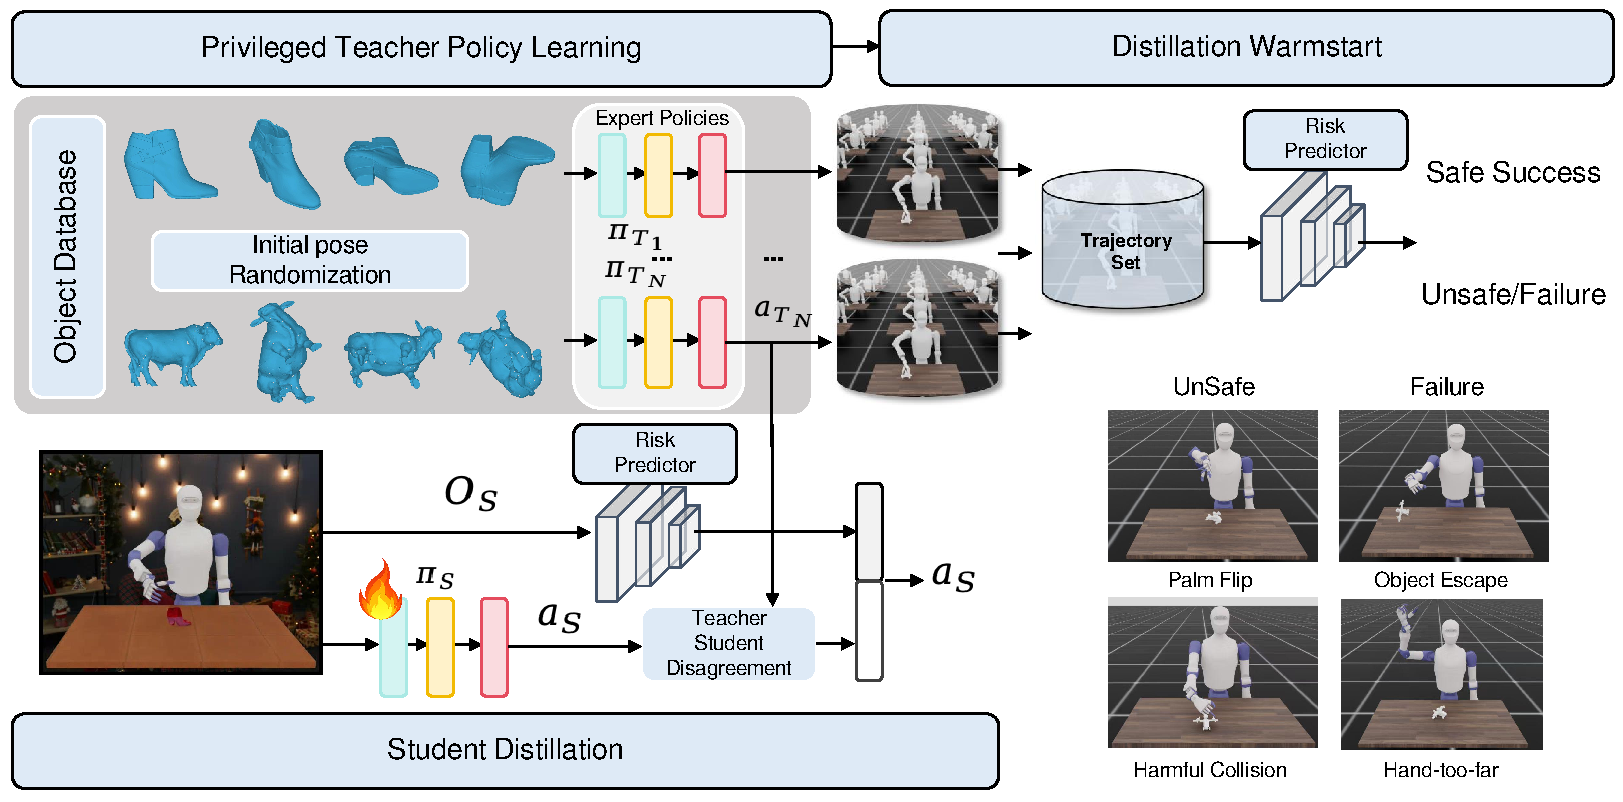
\includegraphics[width=0.8\linewidth]{figures/fig02_network_structure.pdf}
    \par\redtodo{TODO: Update Figure 2.}
    \caption{Overview of the proposed teacher--student learning pipeline. A
    privileged reinforcement learning teacher is trained in simulation and
    subsequently distilled into an RGB-based visuomotor policy for real-world
    deployment. \revision{A vision-language model periodically calibrates the
    intervention thresholds.}}
    \label{fig:pipeline}
\end{figure*}

\subsection{Problem Formulation}
We consider online interactive imitation learning with teacher intervention in a
partially observable Markov decision process (POMDP)
$\mathcal{M}=(\mathcal{S},\mathcal{A},\mathcal{O},P,\Omega,r,\gamma)$, with
privileged teacher state $s_t\in\mathcal{S}$, deployable student observation
$o_t\in\mathcal{O}$ (RGB), action $a_t\in\mathcal{A}$, observation model
$o_t\sim\Omega(\cdot\mid s_t)$, and dynamics
$s_{t+1}\sim P(\cdot\mid s_t,a_t)$. During training, we assume access to a set
of privileged teacher policies $\{\pi_{T_i}\}_{i=1}^{K}$, whereas at deployment
the student policy $\pi_S$ must act solely from $o_t$. Our goal is to distill
the collective teacher behavior into an RGB-based student that achieves high
task success while minimizing unsafe exploration during training.

The induced rollout distribution $p_{\pi_{\mathcal{G}}}$ is defined by the gated rollout policy
$\pi_{\mathcal{G}}$, which switches between the teacher and student policies
according to the intervention gate. Its learning objective and VLM-calibrated
gate are
\begingroup
\small
\begin{equation}
\begin{aligned}
\min_{\substack{\pi_S\in\Pi_S\\ \mathcal{G}\in\mathfrak{G}}}
\;
&
\Bigg[
\underbrace{
-\mathbb{E}_{\tau\sim p_{\pi_{\mathcal{G}}}}\!\left[\mathbb{I}_{\mathrm{succ}}(\tau)\right]
}_{\text{maximize success}}
\;+\;
\lambda\,
\underbrace{
\mathbb{E}_{\tau\sim p_{\pi_{\mathcal{G}}}}\!\left[
\sum_{t=0}^{T-1}\mathbb{I}_{\mathrm{unsafe}}(s_t,a_t)
\right]}_{\text{minimize unsafe}}
\Bigg]
\\
\text{s.t.}\quad
&
a_t=g_t a_t^T+(1-g_t)a_t^S,\\
&
g_t=\mathcal{G}(s_t,o_t)\in\{0,1\},\\
&
s_{t+1}\sim P(\cdot\mid s_t,a_t),\qquad
o_t\sim\Omega(\cdot\mid s_t).
\end{aligned}
\label{eq:vc_objective}
\end{equation}
\endgroup
where $g_t=1$ indicates teacher takeover and $g_t=0$ denotes student control.
\revision{The intervention gate $\mathcal{G}$ and its VLM-calibrated thresholds
are described in Secs.~E--F.}

We formalize task success via a trajectory-level predicate
$\mathbb{I}_{\mathrm{succ}}(\tau)\in\{0,1\}$, which is $1$ if the object is
grasped, lifted, and held above a height threshold for a consecutive duration.
Safety is governed by early termination conditions: letting
$\mathbb{I}_{\mathrm{unsafe}}(s_t,a_t)\in\{0,1\}$ indicate whether any unsafe
event (e.g., harmful collision, object escape, palm flip, hand-too-far) occurs
at time $t$, the trajectory is safe if
$\prod_{t=0}^{T-1}\big(1-\mathbb{I}_{\mathrm{unsafe}}(s_t)\big)=1$.

\subsection{Overview of the Distillation Pipeline}
Fig.~\ref{fig:pipeline} summarizes our teacher--student distillation pipeline,
which consists of three core components: (i) privileged teacher policy training
in simulation (Sec.~C), (ii) risk predictor learning to estimate lift success
under student actions (Sec.~D), and (iii) online student distillation with
teacher intervention (Secs.~E and G). \revision{We additionally introduce a VLM
tuner (Sec.~F) that periodically calibrates the intervention thresholds.} We
warm-start the risk predictor using an offline dataset collected under full
teacher control and continue updating it periodically during online
distillation using mini-batches sampled from a ring replay buffer. During
interactive rollouts, an intervention gate $\mathcal{G}$ switches control
between teacher and student based on an OR-rule combining a learned risk
estimate and teacher--student action disagreement. The student is then
optimized online using per-timestep teacher labels collected under the gated
rollout policy $\pi_{\mathcal{G}}$. \revision{At a slower timescale, the VLM
reviews rollout statistics and representative visual states and proposes
conservative threshold updates.} Pseudo-code is provided in
Alg.~\ref{alg:safe_dagger}.

\begin{algorithm}[t]
\small
\caption{Safe Policy Distillation with Risk-Guided Teacher Intervention}
\label{alg:safe_dagger}
\begin{algorithmic}[1]

\STATE Train teacher policy $\pi_T$ via reinforcement learning
\STATE Collect offline dataset $\mathcal{D}_0$ using $\pi_T$
\STATE Pretrain risk predictor $\hat{Q}(s,a)$ on $\mathcal{D}_0$

\FOR{iteration $k = 1 \dots N$}

    \STATE Observe student observation $o_t$
    \STATE Compute student action $a^S_t \sim \pi_S(\cdot|o_t)$
    \STATE Query teacher action $a^T_t \sim \pi_T(\cdot|s_t)$
    
    \STATE Compute disagreement $\delta_t = \|a^S_t - a^T_t\|_2$
    \STATE Evaluate risk score $\hat{Q}(s_t, a^S_t)$

    \IF{$d_t > \tau_D$ \textbf{or} $\hat{Q}(s_t,a^S_t) < \tau_{\text{success}}$}
        \STATE Execute teacher action $a_t = a^T_t$
    \ELSE
        \STATE Execute student action $a_t = a^S_t$
    \ENDIF

    \STATE Store $(o_t, a^T_t)$ in ring replay buffer $\mathcal{D}$
    \STATE Update student policy $\pi_S$ via imitation loss
    \STATE Update risk predictor $\hat{Q}$ using replay buffer

\ENDFOR

\end{algorithmic}
\end{algorithm}

\subsection{Privileged Teacher Policy Training}
Teacher policy learning is formulated as a reinforcement learning problem with
transition tuples $\langle s_t,a_t,r_t,s_{t+1}\rangle$, where $s_t$ is the
privileged state, $a_t$ is the action, $r_t$ is the reward, and $s_{t+1}$ is the
next state. The objective is to maximize the expected discounted return,
\begingroup
\small
\begin{equation}
\pi_T^*
=
\arg\max_{\pi_T}\;
\mathbb{E}_{\pi_T}
\left[
\sum_{t=0}^{T-1}\gamma^t r_t
\right].
\label{eq:teacher_rl_objective}
\end{equation}
\endgroup
We use a shaped reward $r_t=\sum_{k=1}^{K_r} r_{t,k}$ to encourage stable grasp
acquisition, object lifting, and goal reaching (Table~\ref{tab:reward_terms}).

The teacher is trained in simulation using an asymmetric actor--critic setup
(Table~\ref{tab:teacher_obs}): the actor receives noisy and partial
proprioceptive observations that approximate realistic sensing, while the
critic is provided with privileged full state of both robot and object,
available only in simulation.

\begin{table}[t]
\centering
\footnotesize
\caption{Reward components used for teacher policy training.}
\label{tab:reward_terms}
\setlength{\tabcolsep}{3pt}
\renewcommand{\arraystretch}{0.9}
\resizebox{0.46\textwidth}{!}{%

\begin{tabularx}{\columnwidth}{@{}c l X@{}}
\hline
\textbf{Term} & \textbf{Name} & \textbf{Purpose} \\
\hline
$r_{\text{dist}}$ & Hand distance &
Guides the hand toward the object. \\

$r_{\text{curl}}$ & Finger curl &
Encourages a grasp-ready finger posture. \\

$r_{\text{align}}$ & Palm alignment &
Aligns the palm to a palm-down pose. \\

$r_{\text{contact}}$ & Contact bonus &
Rewards stable thumb--finger contact. \\

$r_{\text{near}}$ & Stay-close &
Keeps the hand near the object after reaching. \\

$r_{\text{goal}}$ & Goal tracking &
Guides the grasped object toward the goal. \\

$r_{\text{lift}}$ & Lift &
Rewards lifting after stable contact. \\

$r_{\text{action}}$ & Action smoothness &
Penalizes abrupt action changes. \\
\hline
\end{tabularx}
}
\end{table}


Episodes terminate at
\begingroup
\small
\begin{equation}
T = \min\left\{t \,\middle|\, \mathbb{I}_{\mathrm{unsafe}}(s_t)=1
\;\;\text{or}\;\; t \ge T_{\max}\right\},
\end{equation}
\endgroup
where $T_{\max}=10\,\mathrm{s}$ is the timeout horizon. Early termination
conditions include palm flip, harmful collision, object escape, and hand-too-far
(see Sec.~A), and are treated as unsafe events for both teacher training and
subsequent intervention decisions.

\subsection{Risk Predictor}
Action disagreement alone cannot anticipate downstream failures, particularly
when the student action is locally similar to the teacher action yet triggers
unstable contact transitions. To address this limitation, we learn a risk
predictor that conservatively estimates the probability of \emph{lift success}.
The predictor is used only during training to guide teacher intervention and is
not required at deployment time.

The risk predictor is designed to estimate risk from multimodal inputs. It
takes as input a state--action pair $(s_t,a_t)$, where $s_t$ comprises robot
proprioceptive features concatenated with image embeddings produced by a visual
encoder to provide semantic information. The visual encoder is trained
end-to-end during distillation and regularized via an auxiliary object-position
prediction loss (Sec.~G). The action $a_t$ is the \emph{executed} action at time
$t$ (teacher or student, depending on the intervention gate). Following a
clipped double-critic design, we maintain two critics $Q_1$ and $Q_2$
implemented as ReLU MLPs with hidden sizes $[256,128]$, each outputting a scalar
logit $z_i(s,a)\in\mathbb{R}$ mapped to a success probability via a
temperature-calibrated sigmoid,
$Q_i(s,a)=\sigma\!\left(z_i(s,a)/T\right)$ for $i\in\{1,2\}$, where $T=4$ is an
empirically set calibration temperature. We then compute
\begingroup
\small
\begin{equation}
\hat Q_{\mathrm{succ}}(s,a)=\min\!\left(Q_1(s,a),\,Q_2(s,a)\right),
\label{eq:success_critic}
\end{equation}
\endgroup
which provides a conservative estimate of lift success (lower values indicate
higher risk).

The predictor is pretrained in a warm-start phase using an offline dataset of
transitions $(s_t,a_t,s_{t+1},a_{t+1},u_t,d_t,h_t)$. Here, $(s_t,a_t)$ and
$(s_{t+1},a_{t+1})$ provide the current and next state--action pairs required by
SARSA-style bootstrapping, $d_t\in\{0,1\}$ is the episode termination flag, and
$h_t\in\{0,1\}$ indicates whether the next action $a_{t+1}$ is defined (valid)
for bootstrapping. The label $u_t\in\{0,1\}$ encodes \emph{safe lift-event}
attainment by time $t$: $u_t=1$ if the object has been lifted above a height
threshold for a consecutive duration (as in $\mathbb{I}_{\mathrm{succ}}$) and no
unsafe event has occurred up to time $t$; otherwise $u_t=0$.

During online distillation, newly collected transitions are appended to a ring
buffer (sized $100k$) at every environment step. The predictor critics are
updated periodically: every $500$ environment steps, we perform $20$ gradient
updates using mini-batches sampled from the buffer using Adam with learning
rate $10^{-3}$.

Training uses SARSA-style bootstrapped regression with an effective termination
signal $d_t^{\mathrm{eff}}=\max(d_t,1-h_t)$ and one-step target
\begingroup
\small
\begin{equation}
y_t=
\operatorname{clip}\!\left(
u_t+\gamma(1-d_t^{\mathrm{eff}})
\min_{i\in\{1,2\}}Q_i^{\mathrm{targ}}(s_{t+1},a_{t+1}),
\,0,\,1\right),
\label{eq:success_target}
\end{equation}
\endgroup
where $Q_i^{\mathrm{targ}}$ are slowly-updated target networks (Polyak
averaging) used only to stabilize bootstrapping, and the $\min$ operator
mitigates overestimation. The critics are optimized with MSE
$\mathcal{L}_{Q_i}=\mathbb{E}\!\left[
w_t\big(Q_i(s_t,a_t)-y_t\big)^2\right]$, with total loss
$\mathcal{L}=\mathcal{L}_{Q_1}+\mathcal{L}_{Q_2}$ and target updates
$\theta'\leftarrow\rho\theta'+(1-\rho)\theta$ ($\rho=0.995$).

During interactive distillation, the predictor estimates the task success
probability of executing the \emph{student} action: given $s_t$ and
$a_t^S\sim\pi_S(\cdot\mid o_t)$, we compute
$\hat Q_{\mathrm{succ}}(s_t,a_t^S)$ and trigger teacher takeover when it falls
below a threshold (Sec.~E).

\subsection{Intervention Mechanism}
At each timestep, we compute (i) a risk score using the learned predictor and
(ii) a teacher--student disagreement score. Disagreement is defined as
$\delta_t\coloneqq\lVert a_t^S-a_t^T\rVert_2$, where
$a_t^T\sim\pi_T(\cdot\mid s_t)$ and $a_t^S\sim\pi_S(\cdot\mid o_t)$ are the
teacher and student action outputs. The risk criterion flags states whose
predicted success under the student action is low, i.e.,
$\hat Q_{\mathrm{succ}}(s_t,a_t^S)<\tau_Q^{(k)}$.

We instantiate the intervention gate $\mathcal{G}$ as an OR-rule that triggers
teacher takeover when either the predictor indicates high risk or the student
deviates substantially from the teacher:
\begingroup
\color{yellow!50!black}
\begingroup
\small
\begin{equation}
g_t=
\mathbb{I}\!\left[
\hat Q_{\mathrm{succ}}(s_t,a_t^S)<\tau_Q^{(k)}
\;\lor\;\delta_t>\tau_{\delta}^{(k)}
\right],
\label{eq:adaptive_gate}
\end{equation}
\endgroup
where $k$ indexes the latest calibration update. Intuitively, disagreement
detects distribution shift, while the risk predictor anticipates downstream
failures even when the instantaneous action discrepancy is small.
\endgroup

\revision{We initialize $\tau_\delta^{(0)}$ to the $90$th percentile of the
teacher--student disagreement $\delta_t$ measured on the warm-start dataset.
We initialize $\tau_Q^{(0)}$ to a low percentile (e.g., the $10$th) of
$\hat Q_{\mathrm{succ}}(s_t,a_t^T)$ computed over successful warm-start
rollouts. These percentiles provide base thresholds chosen empirically to
balance intervention frequency and exploration efficiency; the VLM tuner
subsequently calibrates them during training (Sec.~F).}

\begingroup
\color{yellow!50!black}
\subsection{VLM Threshold Tuner}
\label{subsec:vlm_threshold_tuner}

To adapt the arbitration rule to non-stationary learning dynamics, we introduce
a vision-language-model (VLM) based threshold tuner. The tuner periodically
calibrates the two thresholds in Eq.~\eqref{eq:adaptive_gate} as both the
student policy and the visited-state distribution evolve during data
aggregation. At iteration $k$, the VLM is provided with rollout-level summary
statistics
$\mathcal{C}_k$, including the teacher--student disagreement, predicted
success, intervention frequency, and unsafe-event rate. In addition, it receives
a small set of representative visual observations corresponding to
high-disagreement, low-success, and unsafe states. These visual examples provide
context about the failure modes encountered by the student, while the scalar
statistics summarize the global behavior of the current policy.

The VLM is used as a high-level calibration module. It recommends candidate
thresholds
$(\tilde{\tau}_{\delta}^{(k)},\tilde{\tau}_{Q}^{(k)})$. To avoid abrupt changes, each proposed threshold is constrained around its initial value
and then exponentially smoothed:
\begin{equation}
\begin{aligned}
\tau_{x}^{(k+1)}
&=(1-\alpha)\tau_{x}^{(k)}
+\alpha\,\operatorname{clip}\!\left(
\tilde{\tau}_{x}^{(k)},
c_{x}^{\min}\tau_{x}^{0},
c_{x}^{\max}\tau_{x}^{0}\right),\\[-2pt]
&\hspace{5.5em}x\in\{\delta,Q\}.
\end{aligned}
\label{eq:vlm_threshold_update}
\end{equation}
Here, $\alpha$ controls the adaptation rate, while
$c_{x}^{\min}$ and $c_{x}^{\max}$ define the admissible range relative to the
initial threshold $\tau_x^0$.  
\endgroup


\subsection{Student Policy Distillation}
Student learning is posed as supervised imitation from teacher-labeled
transitions collected under the gated rollout policy $\pi_{\mathcal{G}}$. The
student observes RGB images (two stereo views) together with robot proprioception.

We optimize a combined objective
$\mathcal{L}=\mathcal{L}_{\mathrm{action}}+\mathcal{L}_{\mathrm{aux}}$, where the
auxiliary loss predicts object position to regularize the visual encoder,
$\mathcal{L}_{\mathrm{aux}}=\lVert
\hat{\mathbf{x}}_{\mathrm{obj}}-\mathbf{x}_{\mathrm{obj}}\rVert_2$.

For action imitation, we use a weighted $L_2$ loss,
$\mathcal{L}_{\mathrm{action}}
=\lVert\mathbf{a}_S-\mathbf{a}_T\rVert_W^2
=(\mathbf{a}_S-\mathbf{a}_T)^\top W(\mathbf{a}_S-\mathbf{a}_T)$,
with $W=\mathrm{diag}(w_1,\dots,w_d)$. We set
$w_j=\sigma_{0,j}^{-2}$ using a reference scale $\sigma_{0,j}$ (e.g., the
teacher action standard deviation on dimension $j$), yielding
$\mathcal{L}_{\mathrm{action}}=
\sum_{j=1}^{d}(a_{S,j}-a_{T,j})^2/\sigma_{0,j}^{2}$.

Training proceeds in two stages. (i) \emph{Warm-start:} we collect an offline
dataset (e.g., $100$k transitions) under full teacher control ($g_t\equiv 1$)
to pretrain the risk predictor. (ii) \emph{Online
distillation:} we perform interactive rollouts under $\pi_{\mathcal{G}}$ and
query teacher labels on intervened steps. The student is updated online using
the current-step teacher label only; we do \emph{not} maintain a replay buffer
or DAgger-style aggregated dataset for student updating. The design reduces the
effect of stale supervision and stabilizes online imitation updates.


% \section{Experiment}
% \label{sec:experiment}
% \subsection{Evaluation Metrics}
We designed the following metrics to evaluate both teacher and student policy performance.
Let $\tau\in\{1,\dots,N\}$ index evaluation episodes and $t\in\{0,\dots,T_\tau\}$ index timesteps.
Unless otherwise stated, we run the evaluation episodes with a horizon of 10\,s.

\paragraph{Lift success (ever-lifted with hold).}
Let $h_t^\tau$ be the object height above the table and $H$ a lift threshold. An episode is considered
successful if the object remains above $H$ for at least $N_{\mathrm{hold}}$ consecutive steps. We define
$\mathbb{I}^{\tau}_{\mathrm{lift}}
=\mathbb{I}\!\left[\exists\, t:\ \forall k\in\{0,\dots,N_{\mathrm{hold}}-1\},\ h_{t+k}^{\tau}\ge H\right]$
and report:
$\mathrm{LiftSucc}=\frac{1}{N}\sum_{\tau=1}^{N} \mathbb{I}^{\tau}_{\mathrm{lift}}.$

\paragraph{Unsafe episode rate.}
As stated above, an episode may terminate early due to one of the following conditions:
palm flipped ($\mathbb{I}_{\mathrm{flip}}^{\tau}$), harmful collision ($\mathbb{I}_{\mathrm{coll}}^{\tau}$),
object escape ($\mathbb{I}_{\mathrm{obj}}^{\tau}$), or hand too far ($\mathbb{I}_{\mathrm{hf}}^{\tau}$).
Let $\mathcal{M}=\{\mathrm{coll},\mathrm{obj},\mathrm{flip},\mathrm{hf}\}$ denote the set of termination modes,
and let $\mathbb{I}_m^\tau\in\{0,1\}$ indicate whether mode $m\in\mathcal{M}$ occurs in episode $\tau$.
An episode is unsafe if any termination mode is triggered:
$\mathbb{I}^{\tau}_{\mathrm{unsafe}}
=\mathbb{I}\!\left[\bigvee_{m\in\mathcal{M}} \mathbb{I}^{\tau}_{m}=1\right]$. We report:
$\mathrm{UnsafeRateAvg}=\frac{1}{N}\sum_{\tau=1}^{N} \mathbb{I}^{\tau}_{\mathrm{unsafe}}.$

\paragraph{Failure-mode decomposition.}
Each episode is assigned a single terminal mode $m^\tau\in\mathcal{M}$ from the
set of unsafe events (collision, object escape, palm flip, hand-too-far) as well
as timeout/success where applicable. We define
$\mathbb{I}^{\tau}_{m}=\mathbb{I}[m^\tau=m]$ and report
$\mathrm{FailureModeRate}(m)=\frac{1}{N}\sum_{\tau=1}^{N}\mathbb{I}^{\tau}_{m}, m\in\mathcal{M}.$

When multiple unsafe conditions are triggered in the same timestep, we record
the first triggered termination condition (using a fixed priority order) as the
episode's failure mode.

\subsection{Simulation Experiment Setup}

\begin{figure*}[t]
    \centering
    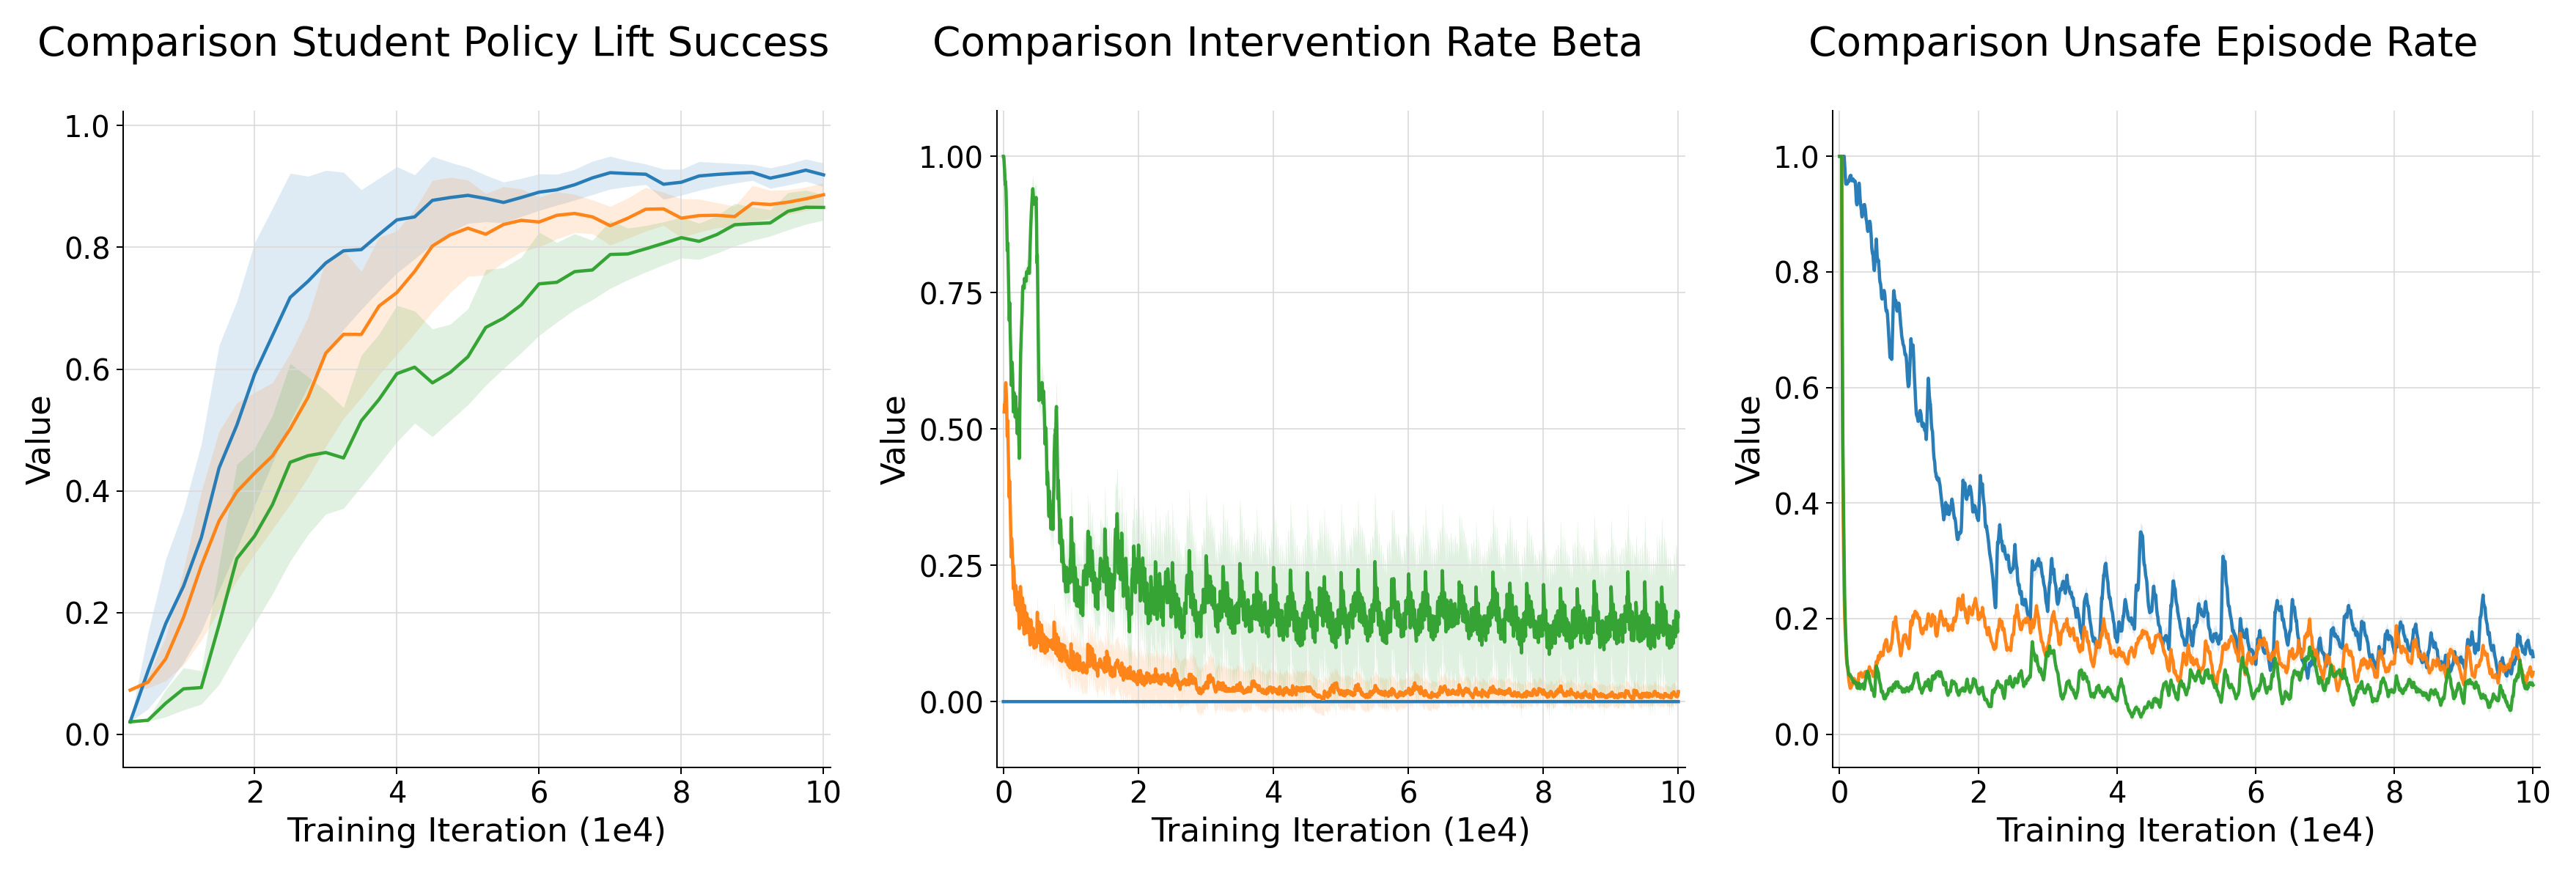
\includegraphics[width=\linewidth]{figures/ablation_comparison.png}
    \caption{\textbf{Ablation studies.}
    The first three panels compare four distillation variants in terms of student lift success, teacher intervention rate $\beta$, and unsafe episode rate, respectively, all plotted over training iterations.
    The rightmost panel shows the VLM-guided trajectory of the intervention operating point over online training.
    Shaded regions indicate variability across runs (mean $\pm$ std).
    Curves correspond to vanilla DAgger (blue), vanilla SafeDAgger (orange),
    \dexsafedagger (green), and \methodname (red).}
    \label{fig:ablation}
\end{figure*}

% The simulation experiments are based on single-arm control of a Tiangong~2 Pro
% humanoid robot equipped with InspireHand RH56DfX dexterous hands. The action
% space is 13-dimensional, consisting of 7 DoF for the robotic arm and 6 DoF for
% the dexterous hand.

% The student policy additionally receives image streams from two cameras at a
% resolution of $320\times240$ pixels and $30$\,fps. The raw stereo images are
% encoded by a visual encoder into a 64-D embedding, which is appended to the
% teacher actor observations to form the student observation. Concretely, the
% visual encoder uses a shared (Siamese) ResNet-18 backbone (last two layers
% removed) for each view, followed by an MLP projection and a 2-layer
% cross-attention transformer to fuse the two views; the resulting
% token is mapped to the 128-dimensional visual feature vector.

% Both teacher policy training and student skill distillation are conducted in Isaac Sim 5.0.0 and
% Isaac Lab 2.2.1 on a single NVIDIA RTX~5090 GPU.

% Forty objects sourced from the Omniverse Asset Library are tested in total. Each teacher policy is trained for 12{,}000 episodes,
% requiring approximately 3.5~hours. The teacher policies achieve a lift success rate ranging from 68\% to 
% 100\% and an unsafe rate ranging from 5\% to 30\%. The results are reported in Table~3.

% During student skill distillation, lighting intensity, direction and background textures are randomized at the
% beginning of each episode. Furthermore, object material properties, textures, and table appearance are randomized to encourage
% improved sim-to-real transfer, following a setup similar to DexTrAH-RGB. The distillation phase requires approximately 2.5~hours to complete
% 100{,}000 episodes.

Simulation experiments use single-arm control on a Tiangong~2 Pro humanoid equipped with InspireHand RH56DfX; the action
space is 13-D (7 arm DoF + 6 hand DoF). The RGB student additionally receives two $320\times240$ camera streams at
30\,fps, encoded by a Siamese ResNet-18 visual backbone with view fusion into a 128-D feature appended to the actor
observation. Teacher training and student distillation are conducted in Isaac Sim 5.0.0 / Isaac Lab 2.2.1 on a single
RTX~5090 GPU.

We evaluate 40 objects from the Omniverse Asset Library and train one
object-specific teacher for each object. Each teacher is trained for
12{,}000 episodes (3.5\,h), totaling 480{,}000 teacher-training
episodes and approximately 140 GPU-hours. Across the 40 teachers, lift-success
rates range from 72--100\%, and unsafe rates range from 5--30\%;
Table~\ref{tab:teacher_perf_200} reports a representative four-object subset.
During distillation, we randomize lighting intensity, direction, background
textures, object material, and table appearance following DexTrAH-RGB-style
domain randomization. The joint student is distilled across all 40 objects for
100{,}000 episodes in 2.5\,h. 

We use GPT-5.5 with high reasoning effort as the VLM. We issue the first VLM
query after 2{,}000 episodes
and subsequently query it every 10{,}000 distillation episodes, resulting in 10
VLM calls over the full 100{,}000-episode training run and approximately
70{,}000 tokens of total usage per run.

% \begin{table}[t]
\centering
\small
\caption{Observation spaces used for teacher RL training under the
asymmetric actor--critic framework.}
\label{tab:teacher_obs}
\resizebox{0.38\textwidth}{!}{%
\begin{tabular}{lcc}
\hline
\textbf{Observation Component} & \textbf{Actor} & \textbf{Critic} \\
\hline
Robot DOF positions  & 13 (noisy) & 13 \\
Robot DOF velocities  & 13 (noisy) & 13 \\
Hand link positions & 18 & 18 \\
Hand link velocities & 18 & 36 (twist) \\
Hand contact forces & -- & 3 \\
Measured joint torque & -- & 19 \\
Object position & 3 & 3 \\
Object rotation (quaternion) & 4 & 4 \\
Object velocity & -- & 6 (twist) \\
Goal position & 3 & 3 \\
Object scale & 1 & 1 \\
Previous actions & 13 & 13 \\
\hline
\textbf{Total dimension} & \textbf{86} & \textbf{132} \\
\hline
\end{tabular}
}
\end{table}

\begin{table}[t]
\centering
\small
\caption{Teacher policy performance on four representative objects from the
40-object training set (200 evaluation episodes per object).}
\label{tab:teacher_perf_200}
\setlength{\tabcolsep}{4pt}
\renewcommand{\arraystretch}{1.2}
\resizebox{0.38\textwidth}{!}{%

\begin{tabular}{l|cccc|c}
\hline
Metric (\%) & WindCart & Boot & ToolBox & Cow & \textbf{Mean} \\
\hline
Lift Success         & 93.5 & 100.0 & 88.5 & 87.0 & 92.3 \\
Unsafe Rate Avg      & 6.5   & 13.5  & 13.5 & 13.5 & 11.8 \\
Harmful collision    & 0.0   & 0.0   & 6.5  & 0.0  & 1.6  \\
Object escape        & 6.5   & 6.5   & 6.5  & 13.5 & 8.3  \\
Palm flipped         & 0.0   & 6.5   & 0.0  & 0.0  & 1.6  \\
Hand too far         & 0.0   & 0.0   & 0.0  & 0.0  & 0.0  \\
\hline
\end{tabular}
}
\end{table}


\subsection{Ablation Studies}

We perform the following ablation studies to validate the design choices in
\methodname and answer four questions: \textbf{(i)~Does our customized RL
recipe produce stronger teachers than the DexTrAH-RGB-style training recipe?}
\textbf{(ii)~Does the intervention mechanism in \dexsafedagger enable safer
exploration during policy distillation?} \textbf{(iii)~Does augmenting action
disagreement with success-value prediction improve the intervention signal?}
\textbf{(iv)~Is visual-language reasoning necessary for adapting the
intervention boundary?}

% \noindent\textbf{(a) DexTrAH-RGB RL teacher + Vanilla DAgger.}
% We follow the DexTrAH-RGB teacher training setup and distill the resulting teacher into a student using
% Vanilla DAgger. Rollouts in simulation are fully controlled by the student policy, while the teacher runs
% in parallel in the background with the intervention rate $\beta$ fixed to $0$. At each timestep, the
% executed student action $a_t^{S}$ is relabeled with the corresponding teacher action $a_t^{T}$.

\noindent\textbf{(a) DexTrAH-RGB RL + Vanilla DAgger.}
The teacher is trained using the DexTrAH-RGB RL recipe and then distilled into
a student policy using supervision only, with no teacher intervention during
rollouts ($\beta=0$).

% \noindent\textbf{(b) Our RL teacher + Vanilla DAgger.}
% We replace the DexTrAH-RGB teacher training pipeline with our customized RL recipe and use the same
% Vanilla DAgger-style online distillation.

\noindent\textbf{(b) Our RL + Vanilla DAgger.}
This setting matches (a), except that our RL recipe replaces the DexTrAH-RGB
teacher-training recipe.

% \noindent\textbf{(c) Our RL teacher + Vanilla SafeDAgger.}
% The teacher policy is trained using our RL pipeline, and we extend Vanilla DAgger to a Vanilla SafeDAgger
% distillation setup. The student and teacher policies are rolled out in parallel, and the teacher action takes
% over only when the $\ell_2$ distance between the teacher and student actions exceeds a threshold, indicating
% a large teacher--student disagreement. The student is trained on teacher-labeled pairs $(o_t^{S}, a_t^{T})$,
% where $o_t^{S}$ denotes the student observation.

\noindent\textbf{(c) Our RL + Vanilla SafeDAgger.}
The teacher training follows the recipe in (b), but we replace Vanilla DAgger
with a disagreement-gated SafeDAgger baseline. The teacher intervenes only when
$\lVert a_t^{T}-a_t^{S}\rVert_2$ exceeds a fixed threshold.

% \noindent\textbf{(d) DexTrAH-RGB RL teacher + SafeDAgger with disagreement and a success-value critic.}
% We follow the DexTrAH-RGB teacher training setup but apply our teacher-intervened distillation pipeline for
% student learning. The teacher and student policies are rolled out in parallel. Teacher intervention is triggered
% when either (i) the teacher disagrees with the student or (ii) the success-value critic flags the current transition
% as unlikely to lead to task success. The intervention decision is computed at every timestep. Likewise, the
% student is trained on teacher-labeled pairs $(o_t^{S}, a_t^{T})$.

\noindent\textbf{(d) DexTrAH-RGB RL + \dexsafedagger.}
We use the teacher-training recipe from (a) and the intervention baseline from
(c), extending it with a Bellman success-value critic under a stationary
intervention policy. Teacher intervention is triggered by either large
teacher--student disagreement or low predicted success.

% \noindent\textbf{(e) Our RL teacher + SafeDAgger with disagreement and a success-value critic.}
% We combine our custom RL pipeline with the proposed teacher intervention mechanism, using both teacher--student
% disagreement and success-value prediction to trigger teacher takeover.

\noindent\textbf{(e) Our RL + \dexsafedagger.}
Following the recipe in (d), we replace the teacher-training pipeline with our
customized RL recipe.

\noindent\textbf{(f) Our RL + \methodname.}
This setting extends (e) by replacing the stationary intervention policy with
the proposed VLM tuner, which periodically calibrates the disagreement-risk
intervention policy using rollout statistics and representative visual states.

\noindent\textbf{(g) Our RL + LLM-DexSafeDagger.}
This setting matches (f), except that the language model receives only the
rollout statistics and no visual observations.

\noindent\textbf{(h) Our RL + Grid-Search \dexsafedagger.}
This setting replaces the language/vision model in (f) with grid search over
the intervention thresholds. The remaining teacher, student, success-value
critic, and distillation components are held fixed.

To answer question~(i), we compare (a) with (b) and (d) with (e). The
DexTrAH-RGB-style RL recipe achieves lower performance than our RL recipe. We
attribute this gap to the specialized tuning of the \textsc{Fabrics} controller
for the original task setup, which transfers poorly to new hardware and
dynamics.

\begin{table}[t]
\centering
\small
\caption{Performance of ablations (a)--(h) on four representative objects from the
40-object training set (200 evaluation episodes per object). Each ablation
reports lift success and average unsafe rate.}
\label{tab:ablation_studies}
\setlength{\tabcolsep}{3pt}
\renewcommand{\arraystretch}{1.15}
\resizebox{0.48\textwidth}{!}{%
\begin{tabular}{l|cc|cc|cc|cc|cc}
\hline
\multirow{2}{*}{Metric (\%)}
& \multicolumn{2}{c|}{WindCart}
& \multicolumn{2}{c|}{Boot}
& \multicolumn{2}{c|}{ToolBox}
& \multicolumn{2}{c|}{Cow}
& \multicolumn{2}{c}{\revisionadded{\textbf{Mean}}} \\
\cline{2-11}
& Lift  & Unsafe
& Lift  & Unsafe
& Lift  & Unsafe
& Lift  & Unsafe
& \revisionadded{Lift}  & \revisionadded{Unsafe}  \\
\hline
\textbf{(a)} & 75.0 & 24.0 & 76.5 & 28.0 & 72.0 & 26.0 & 70.0 & 27.5 & \revisionadded{72.7} & \revisionadded{26.5} \\
\textbf{(b)} & 88.5 & 13.5 & 89.0 & 20.5 & 82.5 & 19.0 & 88.0 & 17.5 & \revisionadded{87.1} & \revisionadded{17.4} \\
\textbf{(c)} & 88.0 & 12.0 & 89.5 & 19.5 & 81.5 & 18.5 & 87.0 & 16.0 & \revisionadded{86.3} & \revisionadded{16.7} \\
\textbf{(d)} & 74.5 & 23.0 & 75.0 & 27.5 & 70.5 & 26.5 & 69.5 & 27.0 & \revisionadded{72.3} & \revisionadded{25.8} \\
\textbf{(e)} & 88.0 & 7.5 & 90.0 & 15.0 & 82.0 & 15.5 & 88.0 & 12.0 & \revisionadded{86.8} & \revisionadded{11.9} \\
\textbf{(f)} & 88.5 & 6.0 & 90.0 & 10.5 & 82.5 & 11.0 & 88.5 & 8.5 & \revisionadded{87.5} & \revisionadded{9.3} \\
\revisionadded{\textbf{(g)}} & \revisionadded{88.0} & \revisionadded{7.5} & \revisionadded{89.5} & \revisionadded{12.5} & \revisionadded{82.0} & \revisionadded{13.0} & \revisionadded{88.0} & \revisionadded{10.5} & \revisionadded{86.9} & \revisionadded{10.2} \\
\revisionadded{\textbf{(h)}} & \revisionadded{86.5} & \revisionadded{7.0} & \revisionadded{88.5} & \revisionadded{14.0} & \revisionadded{81.0} & \revisionadded{13.5} & \revisionadded{87.0} & \revisionadded{11.0} & \revisionadded{85.7} & \revisionadded{11.7} \\
\hline
\end{tabular}
}
\end{table}


\begin{figure*}[!t]
    \centering
    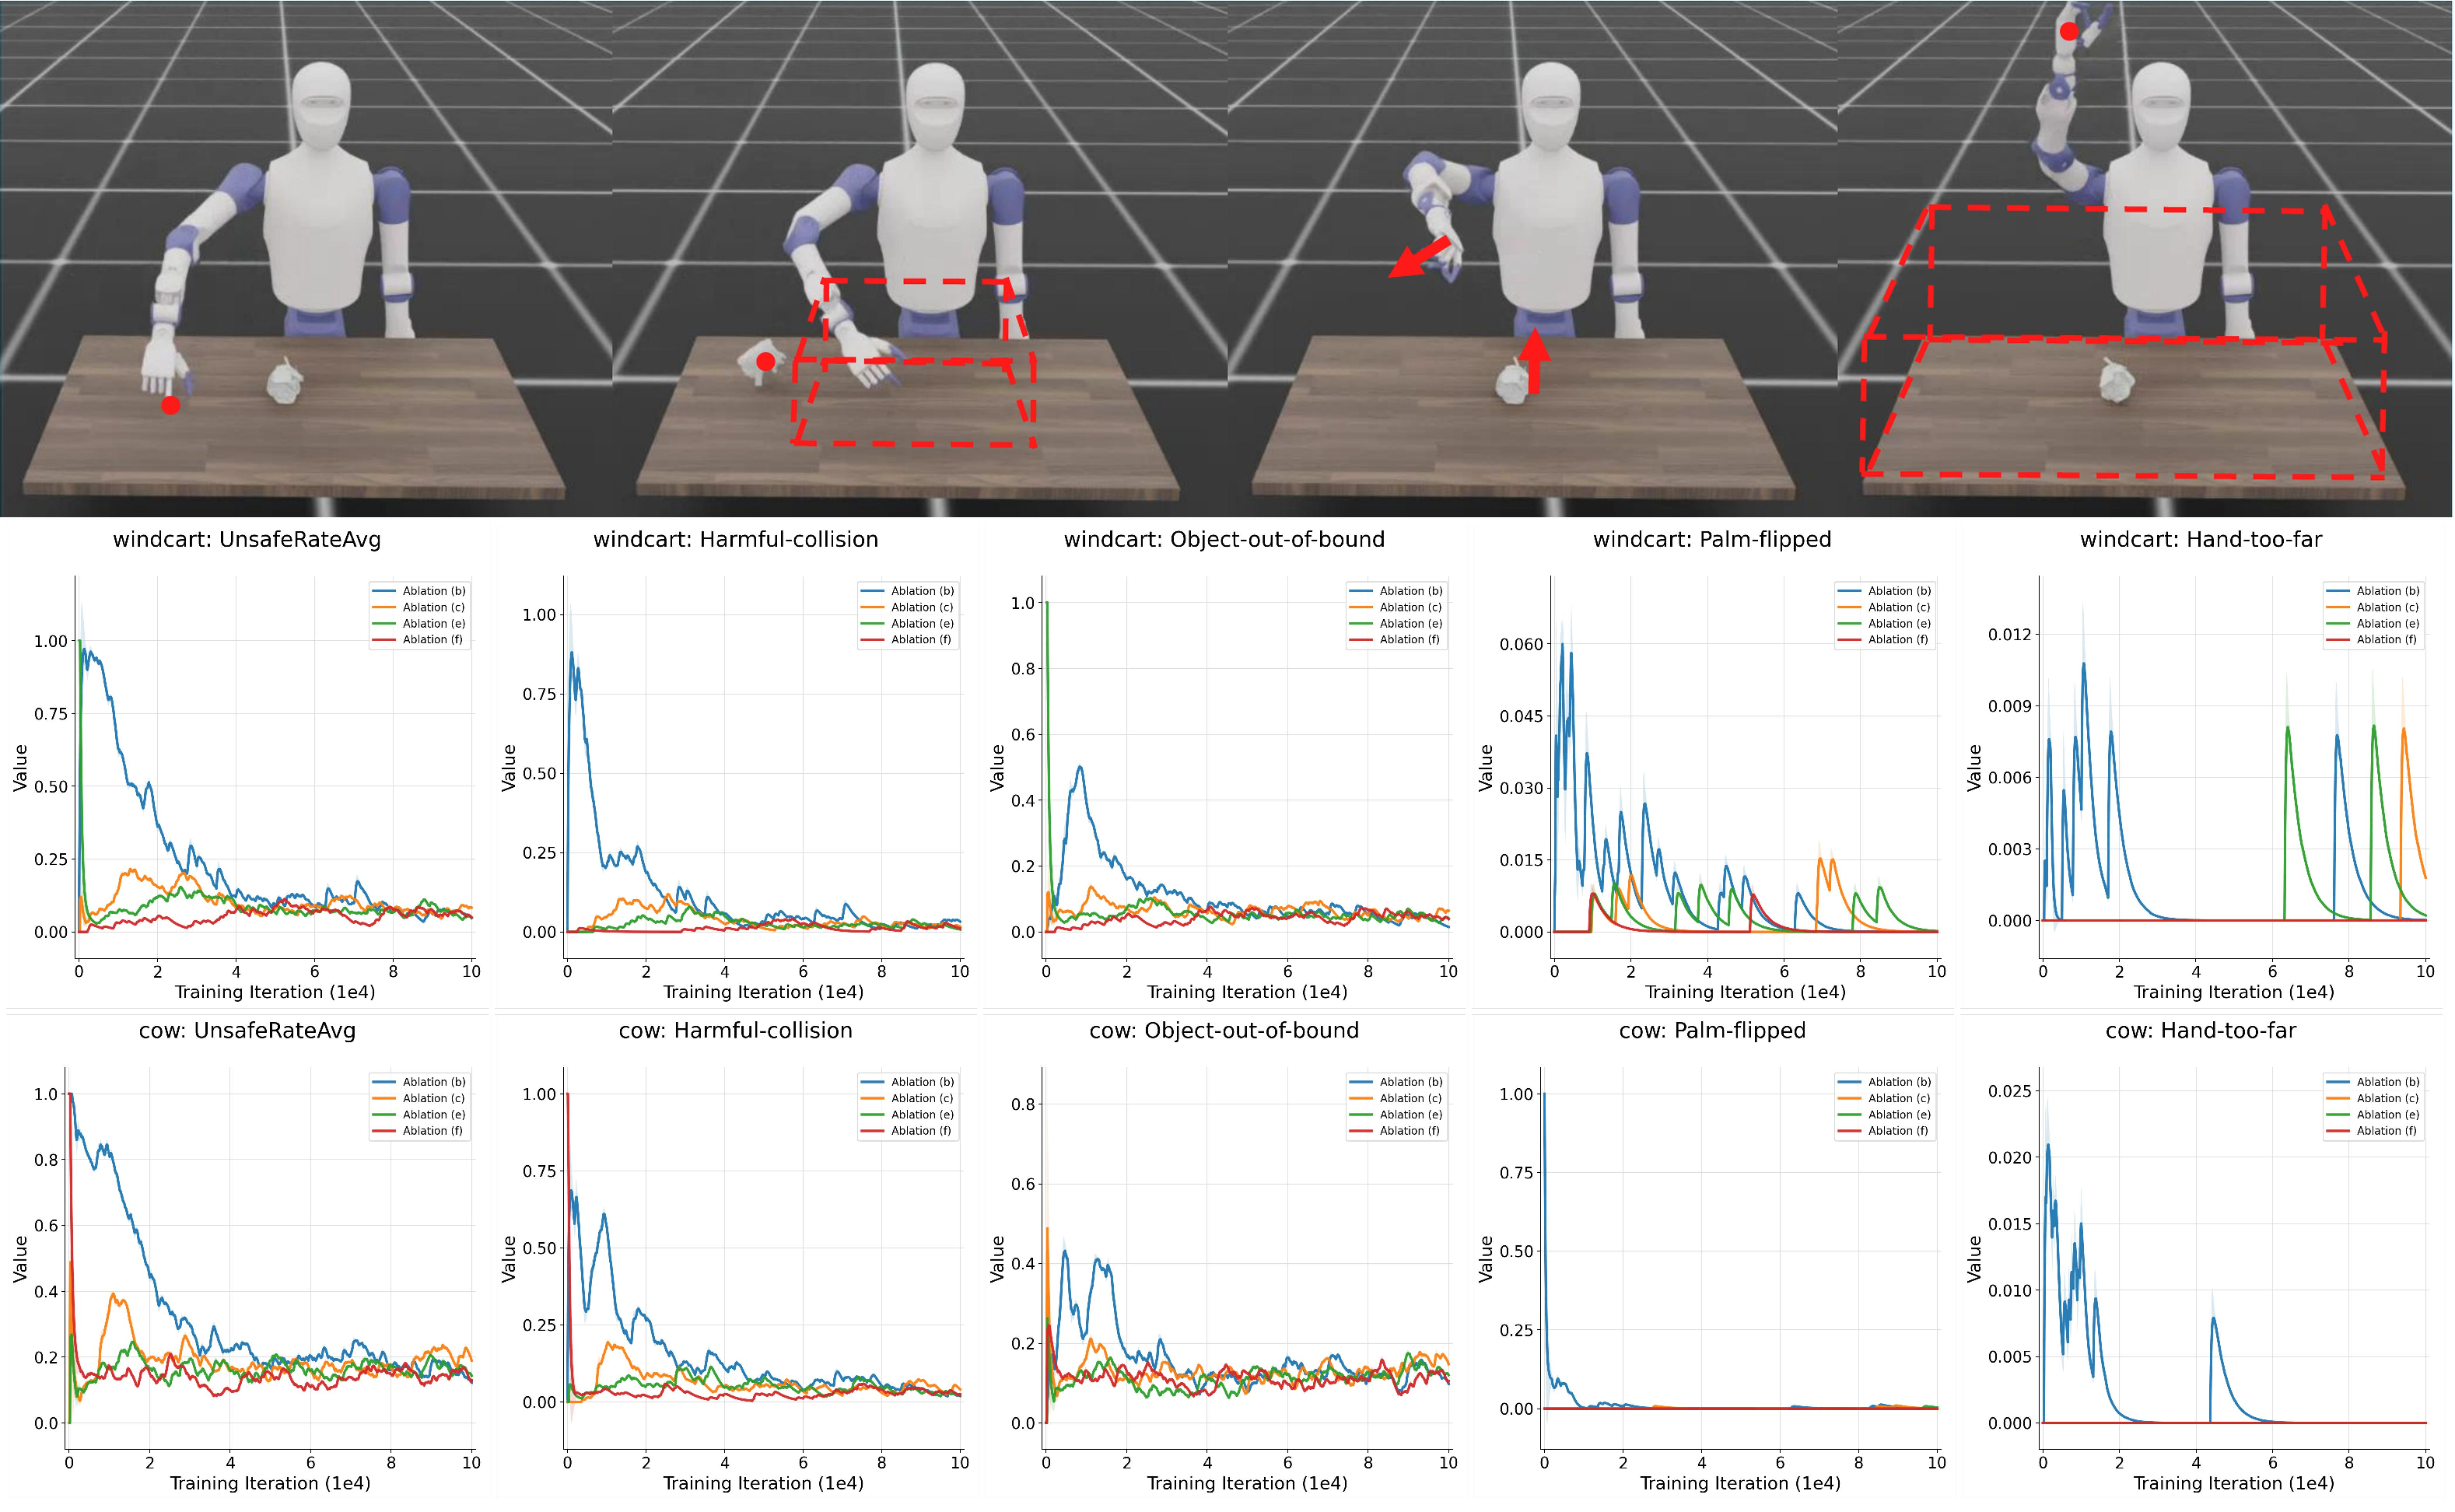
\includegraphics[width=0.82\linewidth]{figures/failure_mode.pdf}
    \caption{\textbf{Per-object failure-mode decomposition during online distillation ablations.}
    We illustrate four task-specific failure modes in simulation (harmful collision, object escape, palm flipped, and hand too far) and report the aggregate unsafe rate together with its per-mode breakdown over training iterations.
    Results are shown for two objects (\texttt{windcart} and \texttt{cow}); lower is better in all plots.
    Curves correspond to four distillation variants: blue, Vanilla DAgger\cite{ross2011reduction};
    orange, Vanilla SafeDAgger\cite{zhang2016query}; green, \dexsafedagger;
    and red, \methodname.}
    \label{fig:failure_modes}
\end{figure*}

We next address question~(ii) by examining the distillation behavior in
Fig.~\ref{fig:ablation}. Ablations (b), (c),
(e), and (f) achieve comparable final lift success
(left), consistent with the intervention policy's focus on safety rather than task success. Unlike
Vanilla DAgger ($\beta=0$), the three intervention variants reduce teacher intervention as the student
improves (middle). They reduce early unsafe episodes by approximately 80\% relative to Vanilla DAgger and
remain below 20\% throughout distillation, with \methodname achieving the lowest rate overall (right).

We address question~(iii) by comparing ablation (c), which uses disagreement alone,
with ablation (e), which adds success-value prediction
while retaining the same RL teacher and stationary intervention policy. The combined gate
intervenes in low-predicted-success states missed by disagreement alone, reducing the average
unsafe-episode rate by about 7.5 percentage points and limiting collision and object-escape
failures without sacrificing task performance. Its unsafe rate approaches the teacher's
average ($\approx 12\%$) by the end of training and reaches a minimum of approximately 8\%.
Fig.~\ref{fig:failure_modes} further shows that harmful collisions and object
escape dominate unsafe episodes. Compared with Vanilla DAgger, all three
intervention variants suppress both failure modes, particularly their early
spikes, demonstrating that teacher intervention limits unsafe exploration
during the initial distillation phase.

\begin{figure}[!t]
    \centering
    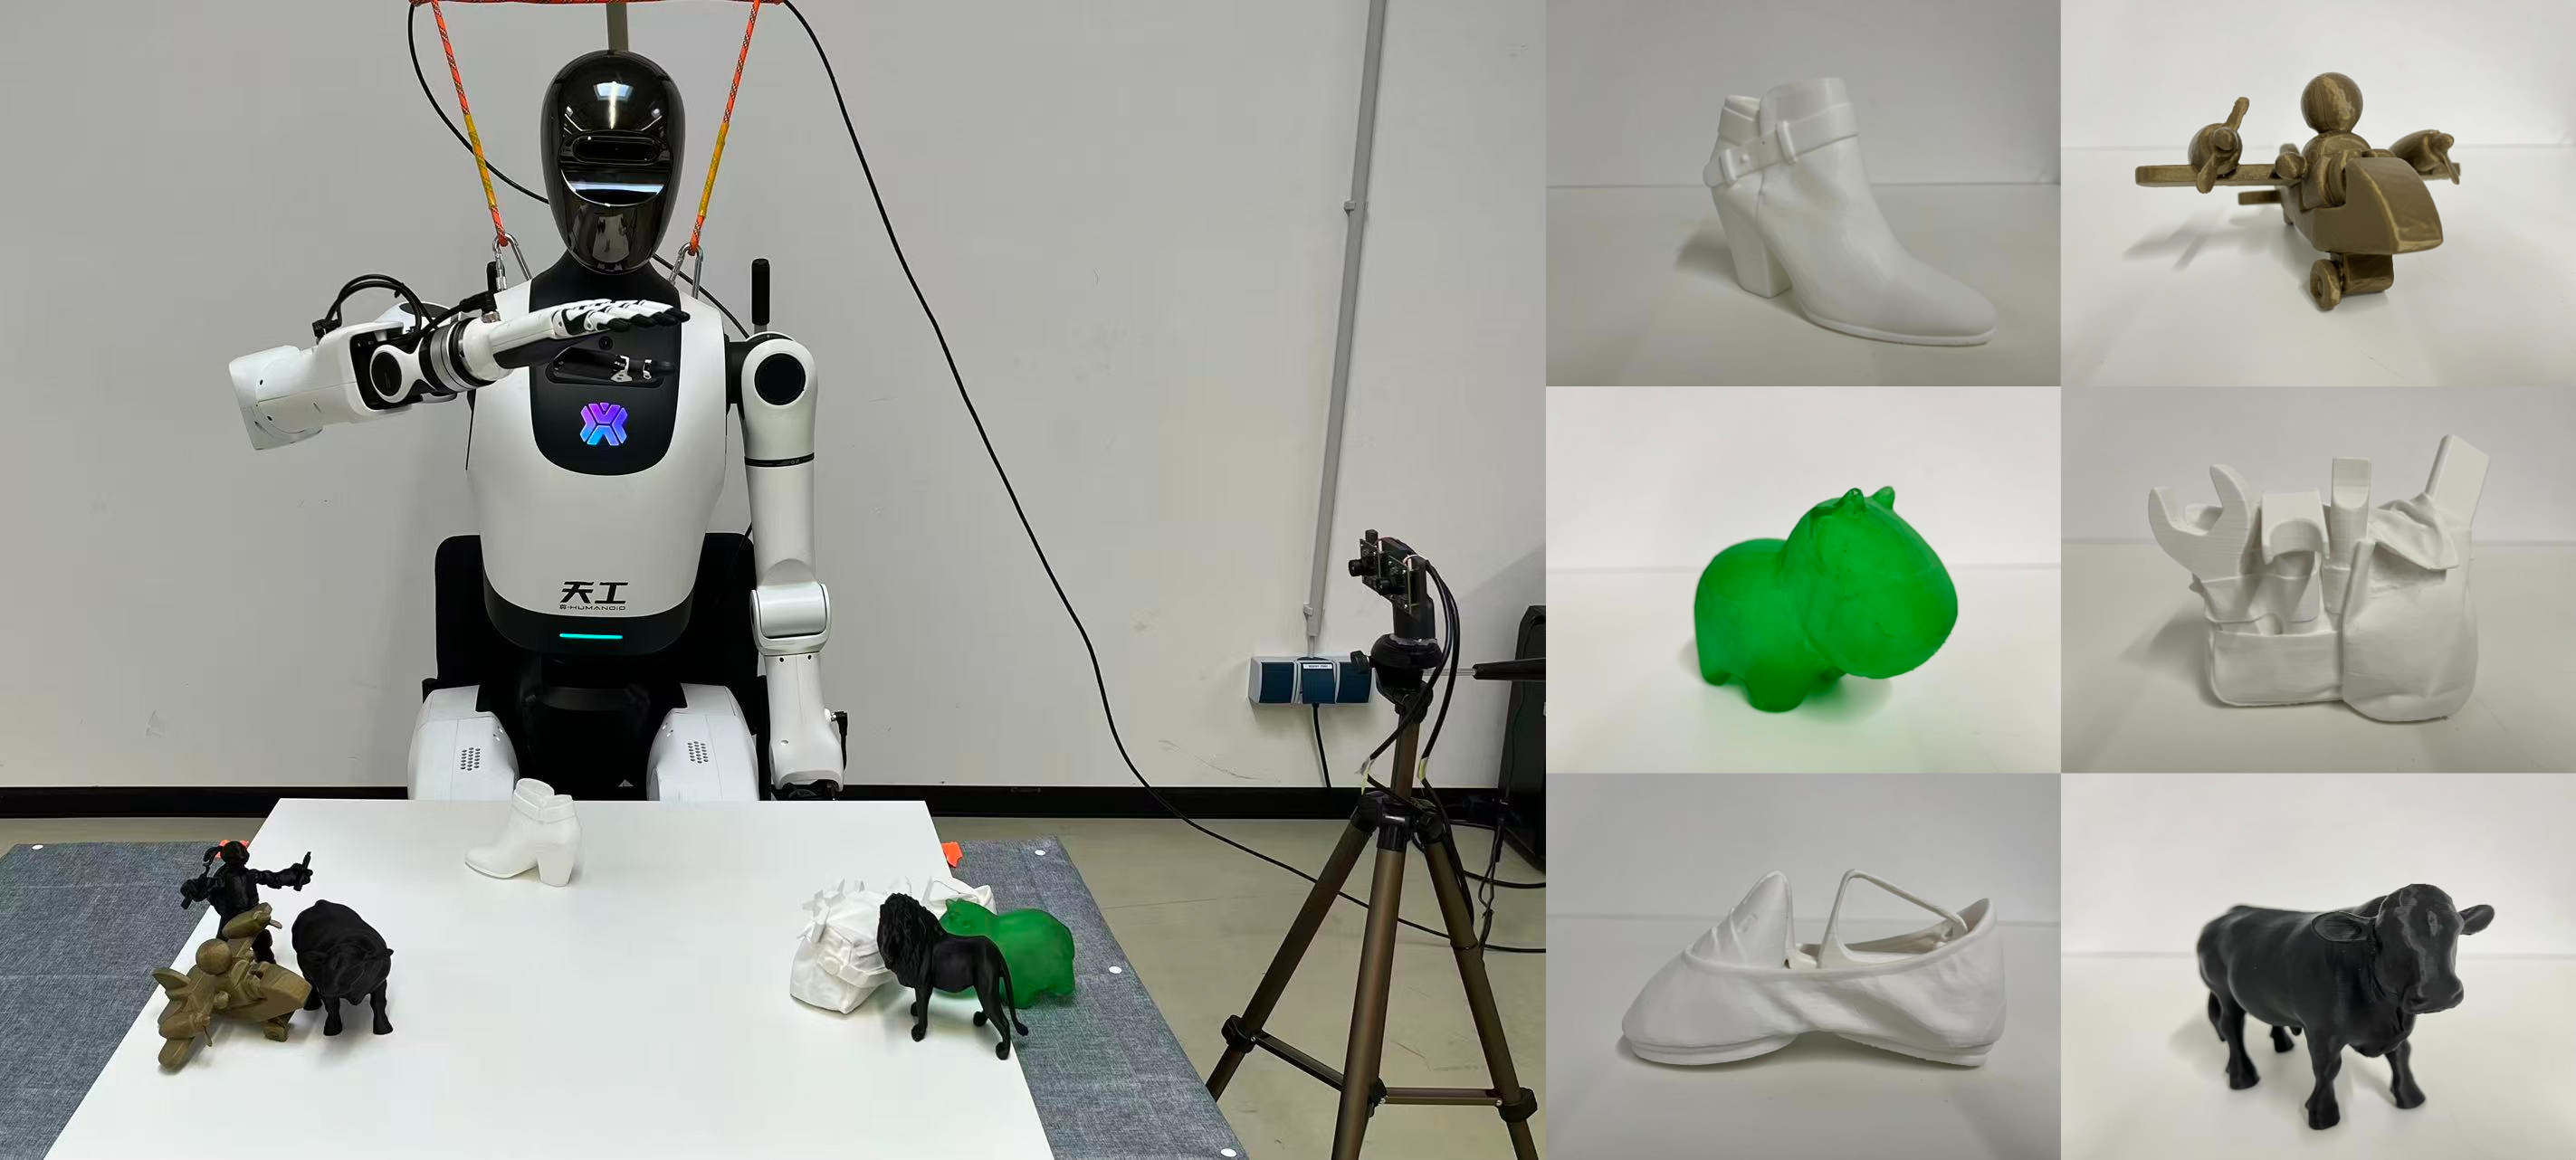
\includegraphics[width=0.85\linewidth]{figures/real_setup_1.png}
    \caption{\textbf{Real-world experimental setup and test objects.}
    Left: the single-arm manipulation platform used for deployment and evaluation.
    Right: examples of the physical objects used in the real-world lift experiments.}
    \label{fig:realworld_exp_setup}
\end{figure}

Finally, we address question~(iv) by comparing ablations (e), (h), (g), and
(f), which form a progression from stationary intervention, to grid-searched
thresholds, to semantics-guided LLM adaptation, and finally to our VLM-guided
recipe. This controlled ladder isolates the contributions of threshold
adaptation, semantic reasoning, and visual context.
\textcolor{red}{TODO: Add the quantitative comparison of ablations (e), (h),
(g), and (f) when the evaluation results are available.}
Across all evaluated
objects, ablation (f) achieves an unsafe-episode rate that is lower than that
of (e) by an average of 4 percentage points, while maintaining comparable lift
success. This result shows that VLM-guided intervention-policy adaptation
improves safety without sacrificing task performance.

\subsection{Real-World Experimental Results}

We evaluate the deployed student policy on 22 objects, comprising 16 seen objects and 6 unseen objects.
Table~\ref{tab:real_world_results} reports a representative six-object subset
and pooled results for the four seen and two unseen objects shown.
The experiments exhibit a lower lift success rate and a higher unsafe episode rate than
the teacher and student evaluation results in simulation, indicating that \methodname does
not fully eliminate the sim-to-real gap. Nevertheless, the resulting policy is sufficiently robust
for real-world deployment.

The unseen-object evaluation reveals a clear generalization gap: compared with
the seen objects shown, the policy's pooled lift success decreases from
\textcolor{red}{85.0\%} to \textcolor{red}{63.3\%}, while its unsafe rate
increases from \textcolor{red}{20.0\%} to \textcolor{red}{40.0\%} on the unseen
objects shown. This degradation is
primarily driven by increased harmful collisions (20.0\% and 26.7\% on Plane and
Shoe), while object escape remains comparable across objects
($\approx$6.7--20.0\%). No palm-flip or hand-too-far events are observed,
suggesting that real-world failures are dominated by contact-rich interactions
rather than gross pose instabilities. Overall, the results indicate that the
remaining sim-to-real gap on unseen geometries is largely attributable to a
contact-strategy mismatch, i.e., the policy fails to adapt its contact
interactions to novel object shapes.

\newcommand{\unseen}[1]{\cellcolor{gray!15}\textbf{#1}}

\begin{table}[t]
\centering
\small
\caption{Representative six-object subset of the 22-object real-world evaluation
(30 episodes per object). The last two columns report pooled results over the
complete sets of 16 seen and 6 unseen objects, respectively. \unseen{Unseen
objects} are shaded.}
\label{tab:real_world_results}
\setlength{\tabcolsep}{4pt}
\renewcommand{\arraystretch}{1.2}
\resizebox{0.48\textwidth}{!}{%

\begin{tabular}{l|cccccc|cc}
\hline
Metric (\%) & WindCart & Boot & ToolBox & Cow & \unseen{Plane} & \unseen{Shoe}
& \makecell{{\textbf{Seen}} \\ {\textbf{avg. (16)}}}
& \unseen{{\makecell{Unseen \\ avg. (6)}}} \\
\hline
Lift Success         & 87.0 & 86.3 & 80.0 & 86.7 & \unseen{66.7} & \unseen{60.0} & 86.2 & \unseen{63.9} \\
Unsafe Rate Avg      & 13.3 & 19.7 & 20.0 & 25.7 & \unseen{40.0} & \unseen{40.0} & 21.2 & \unseen{34.8} \\
Harmful collision    & 0.0  & 6.7  & 13.0 & 13.3 & \unseen{20.0} & \unseen{26.7} & 9.3  & \unseen{20.1} \\
Object escape        & 13.3 & 13.0 & 7.0  & 12.7 & \unseen{20.0} & \unseen{13.3} & 11.9 & \unseen{13.8} \\
Palm flipped         & 0.0  & 0.0  & 0.0  & 0.0  & \unseen{0.0}  & \unseen{0.0}  & 0.0 & \unseen{0.2}  \\
Hand too far         & 0.0  & 0.0  & 0.0  & 0.0  & \unseen{0.0}  & \unseen{0.0}  & 0.0  & \unseen{0.7}  \\
\hline
\end{tabular}
}
\end{table}


% \subsection{Discussion}

% While effectively reducing unsafe exploration, the teacher-intervened online distillation process
% appears to reduce sample efficiency. In Fig.~\ref{fig:ablation}, we observe slower performance growth in
% lift-success evaluation under higher intervention rates. The underlying cause remains unclear; we believe
% there is room for improvement in both exploration safety and sample efficiency within the online
% distillation paradigm.
\label{sec4:expriments}

% \section{Conclusion and Future Work}
% \label{sec:conclusion}
% In this work, we propose \methodname, which integrates
teacher--student disagreement with a Bellman success-value critic trained on
safe-lift-success labels and uses a VLM to adapt the intervention policy.
\methodname improves exploration safety during multi-teacher distillation,
reducing the unsafe-episode rate by \textbf{80\%} relative to the vanilla DAgger
baseline during early training. The introduction of the Bellman critic
reduces the average unsafe-episode rate by \textbf{7.5 percentage points} relative to the
disagreement-only SafeDAgger baseline. In addition, VLM-guided intervention policy adaptation
yields consistent improvements across different visual contexts and unsafe scenarios,
reducing the average unsafe-episode rate by a further \textbf{4 percentage points} relative to
\dexsafedagger.
The proposed method approaches and, in some cases, surpasses the teacher policy's
safety performance. Successful real-world deployment shows that the resulting
student policy partially bridges the sim-to-real gap.

A clear limitation is that performance during distillation, as well as the final student policy, is
largely constrained by teacher capability. Developing a safety-aware teacher training pipeline is a
promising direction for future work to generate stronger teacher policies.



% \bibliographystyle{IEEEtranBST/IEEEtran}
% \bibliography{IEEEtranBST/refs}
{\small
\bibliographystyle{IEEEtran}
\bibliography{IEEEabrv,main}
}

\end{document}
